\documentclass[mf, pdftex]{mgrwms}
\usepackage[utf8]{inputenc}
\usepackage{amsmath}
\newcommand\numberthis{\addtocounter{equation}{1}\tag{\theequation}}
\usepackage{amssymb} 
\usepackage{bbm}
\usepackage{mathtools}
\usepackage{latexsym}
\usepackage{amsthm}
\usepackage{enumerate}
\usepackage{color}
\usepackage[polish]{babel}
\usepackage[OT4]{fontenc}
\usepackage{polski}
\usepackage{graphicx}
\usepackage{float}
\usepackage{placeins}

\graphicspath{{Figs}}
\bibliographystyle{apalike}

\allowdisplaybreaks

\begin{document}

\title{\LARGE Zastosowanie modeli kopułowych do modelowania spreadu aktywów}
\author{Piotr Mikler}
\promotor{dr inż. Jerzy Dzieża}
\nralbumu{409145}
\maketitle
\slowakluczowe{spread, soja, opcje, copuła, vine copula}
\keywords{spread, soybean, option, copula, vine copula}

\newtheorem{thm}{\indent Twierdzenie}[chapter]
\newtheorem{lemma}[thm]{\indent Lemat}
\newtheorem{cor}[thm]{\indent Wniosek}
\newtheorem{obs}[thm]{\indent Obserwacja}
\newtheorem{prop}[thm]{\indent Własność}
\newtheorem{uw}[thm]{\indent Uwaga}
\newtheorem{df}[thm]{Definicja}
\newcommand{\E}{\mathbb{E}}
\newcommand{\R}{\mathbb{R}}
\newcommand{\Pra}{\mathbb{P}}
\newcommand{\1}{\mathbbm{1}}
\newcommand{\Corr}{\text{Cor}}
\newcommand{\Cov}{\text{Cov}}
\newcommand{\Var}{\text{Var}}

\makeatletter
\newcommand*{\defeq}{\mathrel{\rlap{%
                     \raisebox{0.3ex}{$\m@th\cdot$}}%
                     \raisebox{-0.3ex}{$\m@th\cdot$}}%
                     =}
\let\c@table\c@figure
\makeatother


%% --- BODY --- %%
\begin{streszczenie}
	Spready grają dziś ogromną rolę na rynkach finansowych. Służą inwestorom, spekulantom i zarządzającym ryzykiem do oceny potencjalnych zysków z inwestycji, implikowania zmiennych rynkowych, czy kontrolowania ekspozycji na ryzyko. W pracy prezentujemy modele kopułowe jako narzędzia odpowiednie do statystycznej analizy współzależności między komponentami spreadu. 
	
	Literatura bogata jest w przykłady zastosowania dwuwymiarowych kopuł do modelowania dwuwymiarowych spreadów. Te modele, oparte o połączenie analizy szeregów czasowych oraz modelowania reziduów przy pomocy kopuł stały się jednym z klasycznych podejść do problemu wyceny instrumentów pochodnych na spread. Na początku lat 2000 dodatkowo rozwinęła się teoria modeli Vine Copula, pozwalających na elastyczny opis zależności wielowymiarowych. Od tamtego czasu konsekwentnie odnoszą one sukcesy w modelowaniu zjawisk w wielu dziedzinach nauki, od lotnictwa, przez biologię po finanse. Mimo tego, literatura dotycząca aplikacji Vine Copula do modelowania wielowymiarowych spreadów jest zdecydowanie ograniczona. 
	
	Praca poszerza literaturę Vine Copula o aplikację tych modeli do spreadu na 3 aktywa. Prezentujemy niezbędną teorię, oraz pokazujemy w jaki sposób zbudować symulacyjny model dla soybean crush spread, w którym numerycznie wyceniamy europejskie opcje na soybean crush spread. 
\end{streszczenie}

\begin{abstract}
	Nowadays, spreads play a vital role on global financial markets. They serve both investors, speculators and risk managers alike as a measure of potential investment turnover, to imply market variables, or as tools for controlling market risk exposures associated with combinations of risk factors. In this paper, we present copula models as a suitable tool for statistical modelling of dependency between spread components.
	
	The literature is rich with examples of bivariate copulas applied to model bivariate spreads. These models which are a combination of time series analysis and copulas have become one of the classical solutions to the problem of pricing spread derivatives. In early 2000s the copula theory was extended to Vine Copula models, allowing the flexibility of copulas to be used in higher dimensions. Since then they have been successfully applied to model phenomena in a wide range of industries: from aviation to biology to finance. Nevertheless, the literature on modelling spreads in higher dimensions using Vine Copulas is relatively limited.
	
	This paper extends the literature of Vine Copula models by presenting an application to 3-dimensional spread modelling. We present the necessary theory, and show how to build a simulation model for soybean crush spread, as well as how to numerically price European options on that asset.
	
\end{abstract}

\tableofcontents

\begin{wstep}[Wprowadzenie]    % ew. \begin{wstep}[Wprowadzenie]
	Wstep \cite{Bernard_Pricing_Multivariate_Options_with_copulae} example
	
\end{wstep}

\chapter{Wielowymiarowe zmienne losowe}
W klasycznym studium doboru struktury portfela (\cite{Markovitz_MPT}), Markovitz analizuje portfel aktywów. Przedmiotem tej pracy jest opis sposobu, w jaki indywidualne pozycje w portfelu wpływają na jego całościowy zwrot i ryzyko. Współczesna teoria portfela która została zapoczątkowana tą pracą wymaga zamodelowania całego systemu jakim jest zbiór akcji w portfelu. Markovitz pokazuje w swojej pracy istotę współzależności między poszczególnymi aktywami, od której zależy czy ryzyko portfela ulega dywersyfikacji, czy jest amplifikowane. Modelowanie każdego aktywa z osobna jest niewystarczające, ponieważ istota ich wpływu na portfel tkwi w przeważającym stopniu we współzależnościach pomiędzy nimi.\\
Problem wielowymiarowości i poprawnego jej opisu pojawia się nie tylko w finansach, ale w prawie każdej dziedzinie gdzie do realnych problemów aplikuje się modelowanie matematyczne. Zanim wprowadzimy więc pojęcie kopuły, które posłuży nam do analizy wielowymiarowych zależności, w tym rozdziale skupimy się na $d$-wymiarowych wektorach losowych $\mathbf{X} = [X_1, X_2, \dots, X_d]$ i przypomnimy elementy rachunku prawdopodobieństwa i statystyki istotnych z punktu widzenia teorii kopuł.\\

\section{Zmienne losowe}
\label{sec:rozklady_laczne}
Rozpatrywać będziemy przestrzeń probabilistyczną $(\Omega,\mathcal{F},\Pra)$, czyli niech $\Omega$ to pewien niepusty zbiór, $\mathcal{F}$ to $\sigma$-ciało zdarzeń losowych, a $\Pra$ to funkcja $\Pra\colon\Omega\rightarrow[0,1]$. 

\begin{df}[\textit{n}-wymiarowa zmienna losowa]
	\label{df:n_wym_zmienna_losowa}
	\textit{n}-wymiarową zmienną losową nazywamy funkcję określoną na przestrzeni zdarzeń elementarnych $\Omega$ i przyjmującą wartości rzeczywiste:
	
	$$ X\colon \Omega \mapsto \mathbb{R}^{n}, $$

	taką, że
	
	$$ \{ \omega \colon X(\omega) < x) \} \in \mathcal{F},$$
	
	dla każdego $x \in \R.$
\end{df}

W całej pracy zakładać będziemy że poruszamy się w przestrzeni zmiennych ciągłych, ponieważ dotykać będziemy problematyki danych rynkowych o takim charakterze. Teoria kopuł jest rozwinięta co prawda również dla zmiennych dyskretnych (\cite{Genest_Discrete_Copulas}) i dorobiła się już ciekawych aplikacyjnych prac (np. \cite{Koopman_DiscreteCopula_HTF}, czy \cite{Shefzik_Weather}), jednak literatura jest tu zdecydowanie uboższa. Do opisu interesujących nas rozkładów dostępne będziemy więc mieć analityczne postaci ich dystrybuanty lub gęstości. Ponieważ często podaje się różne ich parametryzacje, w tabeli \ref{tab:przykladowe_zmienne_losowe} podajemy gęstości zmiennych losowych przewijających się w tej pracy. Ich wykresy widoczne są na wykresie \ref{fig:przykladowe_zmienne_losowe}.

Warto wspomnieć, że istnieją również użyteczne rozkłady, które nie dają się wyrazić za pomocą gęstości czy dystrybuanty. Najpopularniejszym przykładem mogą być rozkłady stabilne, gdzie jedyne czym może my się posługiwać to funkcja charakterystyczna.  \cite{Stable_Distributions1}, czy \cite{Stable_Distributions2} podają bardzo dobry przegląd teorii rozkładów stabilnych i pokazują ich przewagę w kontekście modelowania nie-gaussowskich zwrotów na rynkach finansowych.

\begin{table}[h]
	\caption{\textbf{Popularne jednowymiarowe zmienne losowe.} Tabela przedstawia dystrybuanty, oraz gęstości popularnych jednowymiarowych zmiennych losowych pojawiających się w tej pracy.}
	\label{tab:przykladowe_zmienne_losowe}
	\centering
	\begin{tabular}{ll|c|c}
		\hline
		\textbf{Rozkład} & \textbf{Oznaczenie} & \textbf{Nośnik} & \textbf{Gęstość} \\
		\hline
		Normalny & $\mathcal{N}(\mu, \sigma)$ & $\mathbb{R}$ & $\frac{1}{\sigma \sqrt{2 \pi}} \exp\big(-\frac{(x-\mu)^2}{2\sigma^2}\big)$\\ 
		T-studenta & $\text{t}(\mu, \sigma, \nu)$ & $\mathbb{R}$ & $ \frac{\Gamma(\frac{\nu + 1}{2})}{\Gamma(\frac{\nu}{2})\sqrt{\pi\nu}\sigma} \bigg[1 + \big(\frac{x - \mu}{\sigma}\big)^2\frac{1}{\nu}\bigg]^{-\frac{\nu + 1}{2}} $ \\ 
		Beta & $\text{Beta}(\alpha, \beta)$ & $[0, 1]$ & $ x^{\alpha - 1}(1 - x)^{\beta - 1}\frac{\Gamma(\alpha + \beta)}{\Gamma(\alpha)\Gamma(\beta)}$ \\ 
		Wykładniczy & $\text{Exp}(\lambda)$ & $\mathbb{R}^{+}$ & $ \lambda e^{-\lambda x}$ \\
		Gamma & $\mathcal{G}(\alpha, \beta)$ & $\mathbb{R}^+$ & $x^{\alpha - 1}e^{-\beta x}\frac{\beta^\alpha}{\Gamma(\alpha)}$\\ 
		
		\hline
	\end{tabular}
\end{table}

\begin{figure}[H]
	\centering
	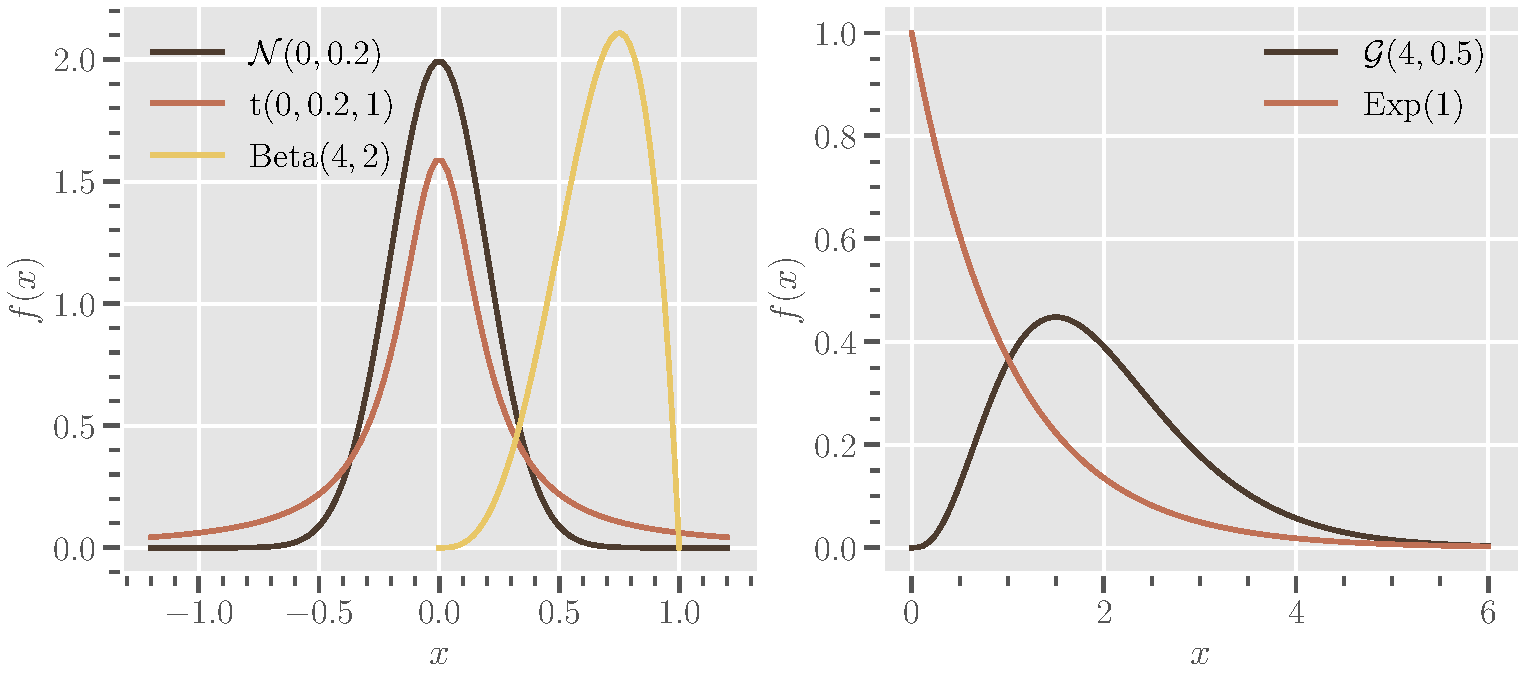
\includegraphics[width=\linewidth]{01_Rozklady_1D}
	\caption{\textbf{Jednowymiarowe zmienne losowe.} Przykładowe gęstości zmiennych losowych z tabeli \ref{tab:przykladowe_zmienne_losowe}.\label{fig:przykladowe_zmienne_losowe}}
\end{figure}

Do opisu zmiennych losowych \emph{wielo}wymiarowych, oprócz gęstości łącznej rozkładu wyróżniamy dodatkowo gęstości warunkowe i brzegowe. Opisują one jak zachowuje się współrzędna wektora losowego, jeśli pozostałe z nich przyjmą pewne wartości, lub jeśli kompletnie wyłączymy ich wpływ.

\begin{df}[Rozkłady brzegowy]
	Rozpatrzmy d-wymiarową zmienną losową $\mathbf{X} = [X_1, X_2, \dots, X_d]$ o gęstości $f(x_1, \dots, x_d)$. Gęstość rozkładu brzegowego $X_j$ definiujemy jako:
	$$f_j(x_j)=\int_{-\infty}^{\infty}\dots\int_{-\infty}^{\infty} f(x_1, \dots, x_{j-1}, x, x_{j+1}, \dots, x_d)  dx_1\dots dx_{j-1} dx_{j+1} \dots dx_d.$$
\end{df}

\begin{df}[Rozkład warunkowy]
	Rozpatrzmy d-wymiarową zmienną losową $\mathbf{X} = [X_1, X_2, \dots, X_d]$ o gęstości $f(x_1, \dots, x_d)$. Gęstość rozkładu warunkowego $X_j \vert X_k$ definiujemy jako:
	$$f_{j|k}(x_j|x_k) = \frac{f(x_1, \dots, x_d)}{f_k(x_k)}.$$
\end{df}


\section{Rozkłady wielowymiarowe}
\label{sec:rozklady_wielowymiarowe}
Naturalnym jest więc, że w praktyce często rozważamy modele wielowymiarowych zmiennych losowych, które mają regularne, łatwe do opisania gęstości łączne. Rozkłady jednowymiarowe z tabeli \ref{tab:przykladowe_zmienne_losowe} w naturalny sposób znajdują swoje rozszerzenia na więcej wymiarów (\cite{MultivariateDistributions}, \cite{Cherubini_Copula_Methods_in_Finance}). Najpopularniejszym tego przykładem jest rodzina $d$-wymiarowych rozkładów eliptycznych, do której należą rozkłady o gęstości postaci:

$$ f_{\mathcal{N}}(x, \mu, \Sigma) = k_d \vert\Sigma\vert^{-0.5}g\big((x-\mu)^T\Sigma^{-1}(x-\mu)\big).$$

W powyższej reprezentacji, $k_d \in\mathbb{R}$ jest stałą zależną od wymiaru, $\mu$ jest $d$-wymiarowym wektorem średnich, $\Sigma \in \mathbb{R}^{d \times d}$ to symetryczna, dodatnio zdefiniowana macierz, a $g \colon [0, \infty) \mapsto [0, \infty)$ jest pewną funkcją która nie zależy od wymiaru wektora.

Dla odpowiednio dobranych $g$ i $k_d$ otrzymamy w tej rodzinie wielowymiarowy rozkład normalny, czy wielowymiarowy rozkład t. Powstają one przy odpowiednio $k_d=(2\pi)^{-0.5d}$ i $g(s) = \exp(-0.5 t)$, lub $k_d=\Gamma(\frac{\nu + d}{2})/\Gamma(\frac{\nu}{2})$ i $g(s) = \big(1 + \frac{t}{\nu})^{-(\nu + d)/2}$.
\begin{figure}[H]
	\centering
	\includegraphics[width=0.45\linewidth]{01_MultivariateGaussian}	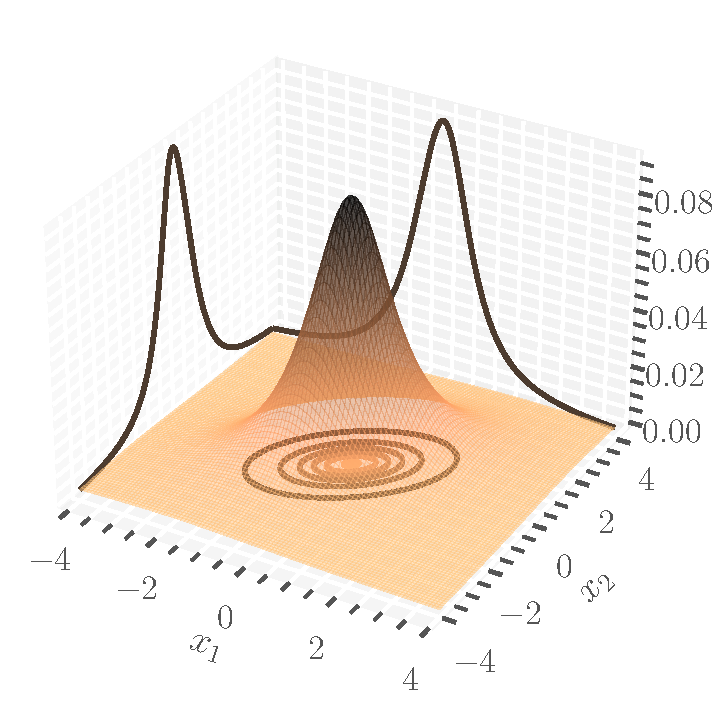
\includegraphics[width=0.45\linewidth]{01_MultivariateStudent}
	\caption{\textbf{Rozkłady eliptyczne.} Gęstości przykładowych rozkładów eliptycznych ($d=2, \mu=[0, 0], \Sigma = \big[\begin{smallmatrix}2&1\\1&2\end{smallmatrix}\big]$). Lewy panel: $2$-wymiarowy rozkład normalny. Prawy panel: $2$-wymiarowy rozkład t ($\nu = 0.5$).\label{fig:multivariate_gaussian_student}}
\end{figure}

Używając rozkładów eliptycznych implikujemy model w którym rozkłady brzegowe pochodzą z tej samej rodziny. Obserwując rysunek \ref{fig:multivariate_gaussian_student}, można rozpoznać charakterystyczne kształty rozkładów brzegowych. Manipulując różnymi rozkładami eliptycznymi możemy więc zamodelować różne struktury korelacji między zmiennymi, czy też ciężkość ogonów, lecz tracimy swobodę wyboru rozkładów brzegowych. \cite{Markovitz_MPT} i jego model bazują właśnie na rozkładzie multinormalnym ponieważ zakładają, że wektor średnich i macierz korelacji wystarczająco opisuje rozkład zwrotów aktywów rynkowych. Podejście to łatwo obalić ze względu na empiryczne dowody ciężkoogonowego charakteru zachowania rynku akcji (\cite{Taleb_BS_is_BS}, \cite{Mandelbrot_NonGaussianity}), czy zjawiska niesymetrycznej, silniejszej korelacji w lewym ogonie (\cite{Taleb_BS_is_BS}, \cite{AssymetricEquityDependency}). Nie mniej jednak nie da się odmówić, że ten prosty model jest wystarczający aby uświadomić jak istotny jest wpływ zależności komponentów na zachowanie całego systemu.\\


\section{Miary współzależności}
\label{sec:miary_współzależności}
Problemem w poprawnym opisie zależności między zmiennymi losowymi jest fakt, że dostępnych mamy wiele statystyk które ją mierzą. Każda z nich uchwyca pewien konkretny aspekt współzależności, i nie da się jasno wyróżnić konkretnej jako ,,najlepszej". W tej sekcji pracy zaprezentujemy wybrane narzędzia służące do badania struktury zależności zmiennych losowych.

\subsubsection{$\rho$ Pearsona}
Podstawową i najbardziej znaną miarą współzależności zmiennych losowych jest korelacja Pearsona.

\begin{df}[Korelacja Pearsona]
	Niech $X$ i $Y$ będą zmiennymi losowymi o skończonych drugich momentach. Współczynnikiem korelacji pearsona $\rho$ nazywamy
	
	$$ \rho(X, Y) \coloneqq \Corr(X,Y) = \frac{\Cov(X,Y)}{\sqrt{\Var(X)}\sqrt{\Var(Y)}}.$$
\end{df}

Ten współczynnik korelacji przyjmuje wartości z zakresu $[-1, 1]$, gdzie $\vert\rho\vert=1$ oznacza idealną liniową relację. Korelacja pearsona jest podstawową miarą zależności podawaną w każdym podręczniku do statystyki. Ma jednak szereg wad: nie jest zdefiniowana dla ciężkoogonowych rozkładów (przez nieokreśloną wariancję), oraz jest wrażliwa na monotonicznie rosnące przekształcenia $X$ i $Y$. Te i wiele innych ograniczeń korelacji pearsona stoi w sprzeczności z aksjomatycznym podejściem do miar zgodności (czyt. \ref{def:miara_zgodnosci}). \\
Gdy w rozdziale \ref{subsec:dwuwymiarowe_kopuly_definicja} zdefiniujemy czym jest główny obiekt tej pracy, czyli kopuła, zależeć nam będzie, żeby móc opisać zależność zmiennych losowych $X$, $Y$ w terminach łączącej je kopuły $C$. Z tego powodu, interesujące dla nas będą miary zależności, które są niezmiennicze na monotonicznie rosnące przekształcenia (ze względu na transformację PIT \ref{def:PIT}, czyt. rozdział \ref{subsec:dwuwymiarowe_kopuly_definicja}). Korelacja pearsona nam tego nie zapewni, ale możemy zdefiniować inne miary: zgodności zmiennych losowych, które posiadają lepsze własności z punktu widzenia teorii kopuł.\\

Aby w pełni zdefiniować aksjomatyczne podejście do miar zgodności jak wprowadził to Scarsini w \cite{Scarsini1984}, potrzebujemy mieć dostępne pojęcie kopuły. W tej pracy formalnie zostaną one wprowadzone dopiero w definicji \ref{def:bivariate_copula}, w związku z czym na ten moment powiemy jedynie (nieformalnie), że kopuła jest funkcją która opisuje charakter i siłę zależności między zmiennymi losowymi. Pełną definicję i opis czym są kopuły można przeczytać w rozdziale \ref{sec:dwuwymiarowe_kopuly}.

\begin{df}[Miara zgodności]
	Rozpatrzmy zmienne losowe $X$ i $Y$ powiązane kopułą $C$. $M_{X,Y}=M_C$ nazwiemy miarą zgodności, wtedy i tylko wtedy gdy:
	\begin{enumerate}
		\item jest zdefiniowana dla dowolnych zmiennych $X$, $Y$
		\item jest relatywna, lub znormalizowana: $M_{X,Y}\in[-1,1]$
		\item jest symetryczna: $M_{X,Y}=M_{Y,X}$
		\item jeśli $X$ i $Y$ są niezależne, to $M_{X,Y}=0$
		\item $M_{-X,Y}=M_{X,-Y}=-M_{Y,X}$
		\item jest zbieżna, gdy kopuła jest punktowo zbieżna, tzn. jeśli $\{(X_n,Y_n)\}$ jest ciągiem ciągłych zmiennych losowych o kopułach $\{C_n\}$, oraz 
		$$ \lim\limits_{n\to\infty} C_n(u, v) =C(u, v)\text{, dla każdych }(u, v)\in[0,1]^2,$$
		to wtedy
		$$ \lim\limits_{n\to\infty}M_{X_n,Y_n}=M_{X,Y}.$$
		\item przestrzega relacji zgodności: jeśli $C_1(u,v) \leqslant C_2(u,v)$ dla wszystkich $(u, v)\in[0,1]^2$, to $M_{C_1} \leqslant M_{C_2}.$
	\end{enumerate}
	\label{def:miara_zgodnosci}		
\end{df}

Aksjomatyczne podejście z powyższej definicji zawęża przestrzeń miar zgodności do takich, które są niezmiennicze względem rosnących transformacji, czyli:
$$ M_{X,Y} = M_{\alpha(X), \beta(Y)},$$
dla dowolnych funkcji $\alpha,\beta$ rosnących prawie wszędzie.\\

\subsubsection{Współmonotoniczność i przeciwmonotoniczność}
Współmonotoniczność i przeciwmonotoniczność to szczególne przypadki zależności zmiennych losowych, w których są one od siebie perfekcyjnie zależne.

\begin{df}[Zbiór współmonotoniczny]
	Zbiór $A \subset \R^2$ nazywamy współmonotonicznym, wtedy i tylko wtedy gdy dla dowolnych $(x_1, y_1)$, $(x_2, y_2)$ z $A$ zachodzi:
	
	$$ (x_1 - y_1)(x_2 - y_2) >0.$$
\end{df}

\begin{df}[Zbiór przeciwmonotoniczny]
	Zbiór $A \subset \R^2$ nazywamy przeciwmonotonicznym, wtedy i tylko wtedy gdy dla dowolnych $(x_1, y_1)$, $(x_2, y_2)$ z $A$ zachodzi:
	
	$$ (x_1 - y_1)(x_2 - y_2) <0.$$
\end{df}


\begin{df}[Zmienne losowe współ- i przeciwmonotoniczne]
	Wektor losowy $(X, Y)$ nazywamy współmonotonicznym (przeciwmonotonicznym), lub perfekcyjnie dodatnio (ujemnie) zależnym wtedy i tylko wtedy gdy istnieje zbiór współmonotoniczny (przeciwmonotoniczny) $A\subset\R^2$:
	
	$$ \Pra[(X,Y)\in A]=1.$$
\end{df}

Współmonotoniczność i przeciwmonotoniczność zmiennych losowych jest ważnym konceptem w teorii kopuł, ponieważ definiuje najsilniejszy rodzaj zależności jakie kopuły mogą reprezentować (czyt. twierdzenie \ref{thm:frechet_hoeffding}).

\subsubsection{$\tau$ Kendalla i $\rho$ Spearmana}

Współczynniki $\tau$ Kendalla i $\rho$ Spearmana oba spełniają aksjomaty miar zgodności z \cite{Scarsini1984}. Są współczynnikami rangowymi, więc nie zależą od monotonicznych przekształceń rozkładów brzegowych $X$ czy $Y$. Ich zaletą jest to, że mogą być przez to jednoznacznie przedstawione w języku kopuły - co znajduje zastosowanie przy estymacji parametrów modeli kopułowych. Ta własność zazwyczaj nie zachodzi w przypadku korelacji Pearsona.

\begin{df}[$\tau$ Kendalla]
	Współczynnik $\tau$ Kendalla między ciągłymi zmiennymi losowymi $X$ i $Y$ o kopule definiujemy jako:
	$$ \tau = \Pra[(X_1-X_2)(Y_1-Y_2)>0] - \Pra[(X_1-X_2)(Y_1-Y_2) <0], $$
	gdzie $(X_1, Y_1)$ i $(X_2, Y_2)$ są kopiami iid wektora $(X, Y)$.
\end{df}

\begin{df}[$\rho$ Spearmana]
	Współczynnik $\rho$ Spearmana między ciągłymi zmiennymi losowymi $X$ i $Y$ o rozkładach brzegowych $F_X$ i $F_y$ zadany jest przez:
	$$ \rho = \Corr[F_X(X), F_Y(Y)].$$
\end{df}

Współczynniki te dają się jednoznacznie wyrazić za pomocą kopuł łączących $X$~i~$Y$~-~własność tę podamy w rozdziale \ref{subsec:dwuwymiarowe_kopuly_definicja}. Istotny również jest fakt, że ich ekstremalne wartości, tj. $\rho= 1$, czy $\tau=1$ odpowiadają współmonotoniczności zmiennych losowych, a $\rho=-1$, czy $\tau=-1$ odpowiadają przeciwmonotoniczności.

\subsubsection{Zależność ogonów}
Na zależność zmiennych losowych można popatrzeć również ze strony zależności obserwacji ekstremalnych. Rozważmy następującą statystykę:

\begin{df}[Współczynnik zależności ogonów]
	Górnym współczynnikiem zależności ogonów $(X_1, X_2)$ o rozkładach brzegowych $F_1$ i $F_2$ i kopuli $C$ nazywamy:
	$$ \lambda^{u} = \lim\limits_{t\to1^{-}}\Pra[X_2 > F_2^{-1}(t) \vert X_1 > F_1^{-1}(t) ].$$
	Dolnym współczynnikiem nazywamy:
	$$ \lambda^{l} = \lim\limits_{t\to0^{+}}\Pra[X_2 \leqslant F_2^{-1}(t) \vert X_1 \leqslant F_1^{-1}(t) ].$$
\end{df}

Współczynniki zależności ogonów informują o sile zależności zmiennych losowych w granicy, gdy dążymy z jedną z nich coraz dalej w jej ogon. Mówimy, że zmienne losowe posiadają zależność ogonów jeśli $\lambda \in (0, 1]$, lub jej nie posiadają gdy $\lambda =0$. Te wspołczynniki zależą przede wszystkim od obserwacji będących ekstremalnymi względem obu zmiennych. Rysunek \ref{fig:tail_dependence} prezentuje przykładowy rozkład posiadający dolny współczynnik zależności ogonów, lecz nie posiadający górnego wspołczynnika. Kolorami zaznaczone są obserwacje które wpływają na dolny (szare punkty) i górny (czerwone punkty) współczynnik zależności ogonów.\\
W praktycznych zastosowaniach, jest on jednak trudny do kalibracji z danych - koncept ten działa raczej w drugą stronę: z parametrów skalibrowanego modelu implikowany jest współczynnik zależności ogonów.
\begin{figure}[H]
	\centering
	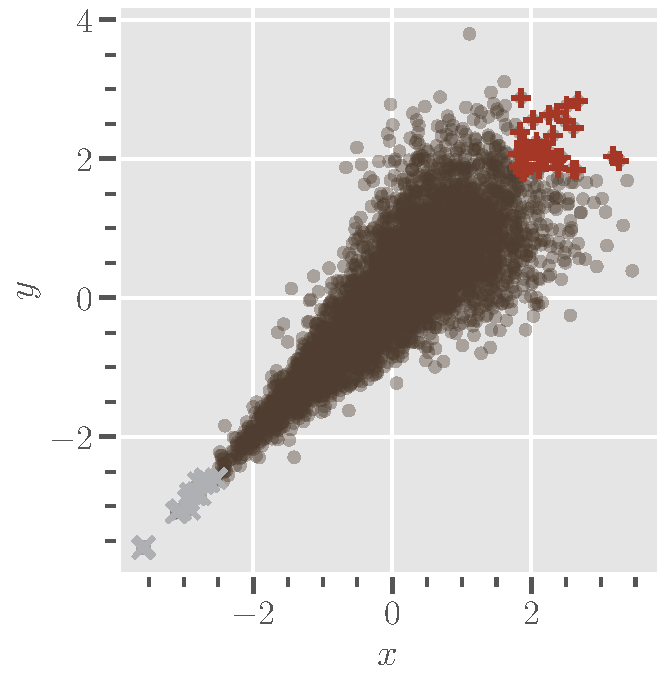
\includegraphics[width=0.5\linewidth]{01_Tail_dependence}	
	\caption{\textbf{Współczynnik zależności ogonów.} Rozkład o dolnym współczynniku i braku górnego współczynnika. Obserwacje zaznaczone na szaro wpływają na dolny współczynnik. Obserwacje zaznaczone na czerwono wpływają na górny współczynnik zależności ogonów.\label{fig:tail_dependence}}
\end{figure}

W tym rozdziale zdefiniowialiśmy różne miary pomagające nam zrozumieć zależność zmiennych losowych. Widzimy zatem, że korelacja Pearsona i modele eliptyczne to za mało, aby w pełni uchwycić charakter współzależności. W kolejnym rozdziale podamy teorię \emph{kopuł}, które dadzą nam odpowiednie narzędzia do walki z tym problemem.


\mgrclosechapter
\chapter{Modele kopułowe}
\label{ch:modele_kopulowe}
Zgodnie z drugim filarem Basel II instytucje finansowe zobowiązane są dokonywać regularnych symulacji stress testowych, podczas których ich kondycja finansowa poddawana jest ekstremalnym negatywnym ruchom rynkowym. Ma to na celu postawienie instytucji przed hipotetycznym kryzysowym scenariuszem i ocenę czy instytucja ma zgromadzoną wystarczającą ilość kapitału ekonomicznego aby przetrwać taką sytuację (\cite{BaselII}). Podczas symulacji stress testowych, regulator podaje instytucjom ogólny scenariusz rynkowy w postaci trajektorii pewnych wiodących zmiennych makroekonomicznych. Każda instytucja musi następnie zinterpretować zadany scenariusz i rozszerzyć go na zbiór zmiennych istotnych z punktu widzenia ich biznesu. Standardową praktyką w tym procesie, nazywanym \emph{shock expansion}, wciąż są modele ekonometryczne, wynikiem których są w większości pojedyncze trajektorie. \cite{Siddique_Stress_testing}\\
Podejście to ma istotną wadę: nie jesteśmy w nim w stanie podać prawdopodobieństwa wystąpienia takiej realizacji \emph{shock expansion}, ponieważ wynikiem są jedynie pojedyncze trajektorie. Nowym kierunkiem w procesie \textit{shock expansion} zaczyna być natomiast tzw. probabilistic stress testing (np. \cite{Aste_Probabilistic_Stress_Testing}). Ideą jest tu zamodelowanie wielowymiarowego systemu zmiennych makroekonomicznych i rynkowych, w sposób pozwalający zaaplikowanie rynkowej narracji regulatora jako zbioru warunkującego ten system. Umożliwia to odzyskanie rozkładów warunkowych dla innych komponentów systemu, w szczególności dla tych które są potrzebne jako wynik \emph{shock expansion}.\\
\cite{Aste_Probabilistic_Stress_Testing} w swojej pracy bada potencjalne zastosowanie rozkładów eliptycznych, wprowadzonych w rozdziale \ref{sec:rozklady_laczne} jako jednego, wielowymiarowego modelu wyżej opisanego systemu. Wyniki które otrzymuje wskazują, że mimo iż rozkłady eliptyczne dają intuicyjne wyniki co do ogólnego kierunku rozwoju warunkowanych rozkładów, to nie są wystarczająco elastyczne aby poprawnie uchwycić wszystkie cechy systemu. Jako tego powód, Aste wymienia \textit{symetrię} modelu, która przejawia się w konieczności wyboru tych samych rodzin rozkładów brzegowych i jest implikowana użyciem rozkładów eliptycznych.\\

Powyższy przykład to jeden z długiego szeregu który ilustruje, że praktyczne problemy wymagają dowolności w wyborze rozkładów brzegowych (wiele innych interesujących przykładów podają \cite{Cherubini_Copula_Methods_in_Finance}, czy \cite{Cherubini_Dynamic_Copula_Methods_in_Finance}). Dlatego mimo, że istnieje wiele matematycznie poprawnych rozszerzeń zmiennych losowych z $d=1$ do $d>2$ (jak wielowymiarowy rozkład normalny, wielowymiarowy rozkład t-Studenta, wielowymiarowy rozkład gamma, etc.), to nie cieszą się one dużym zastosowaniem w praktyce. Odpowiedzią na to ograniczenie są kopuły - modele wielowymiarowych zmiennych losowych, pozwalające na oddzielenie wpływu rozkładów brzegowych od wpływu struktury zależności na cały system.\\

\section{Dwuwymiarowe kopuły}
\label{sec:dwuwymiarowe_kopuly}
\subsection{Wprowadzenie i definicja}
Teorię kopuł zapoczątkował Abe Sklar w \cite{Sklar_Theorem}, podając następujące twierdzenie:

\begin{thm}[Twierdzenie Sklara]
	Niech $X_1, X_2, \dots, X_d$ będą zmiennymi losowymi ciągłymi, o dystrybuantach $F_1, \dots, F_d$, i rozkładzie łącznym z dystrybuantą $F$. Wtedy istnieje unikalna \emph{kopuła} $C$, taka że dla wszystkich $\mathbf{x} = (x_1, \dots, x_d) \in \mathbb{R}^n$:
	\begin{equation}
		F(x_1, \dots, x_d) = C(F_1(x_1), \dots, F_d(x_d)).
		\label{eq:sklar_theorem}
	\end{equation}
	
	Zachodzi również twierdzenie odwrotne: Mając dowolne dystrybuanty $F_1, \dots, F_d$ i kopułę $C$, funkcja $F$ zdefiniowana według \ref{eq:sklar_theorem} jest d-wymiarową dystrybuantą, o rozkładach brzegowych $F_1, \dots, F_d$. 
	\label{thm:sklar_theorem}
\end{thm}

Twierdzenie \ref{thm:sklar_theorem} przede wszystkim podaje więc algorytm postępowania mówiący w jaki sposób otrzymać wielowymiarowy rozkład o dowolnie wybranych, potencjalnie różnych rozkładach brzegowych. Dodatkowo, Sklar stwierdza istnienie pewnego obiektu, nazwanego kopułą/funkcją łączącą (łac.\emph{copulae}: łączyć) który jest jednoznacznie zdefiniowany dla dowolnego ciągłego rozkładu wielowymiarowego, w taki sposób, że rozkład łączny da się przedstawić jako tę funkcję zaaplikowaną do rozkładów brzegowych.\\

Oczywistym jest, że nie wszystkie wielowymiarowe funkcje mogą pełnić taką rolę. Rozważymy więc jakie warunki musi spełniać $C$ z twierdzenia \ref{thm:sklar_theorem}, aby mogła być kopułą.
\begin{df}[Grounded function]
	Rozważmy $A_1$ i $A_2$ - dwa niepuste podzbiory $\mathbb{R}$, oraz funkcję $G\colon A_1\times A_2\mapsto\mathbb{R}$. Niech $a_i$ oznacza najmniejszy element $A_i$, dla $i=1, 2$. Funkcję $G$ będziemy nazywać uziemioną \emph{(eng. grounded)}, jeśli dla każdej pary $(v, z)$ z $A_1\times A_2$,
	\begin{equation}
		G(a_1, z) = 0 = G(v, a_2).
	\end{equation}
	\label{def:grounded_function}
\end{df}

\begin{df}[2-increasing function]
	$G\colon A_1\times A_2\mapsto \mathbb{R}$ nazywamy dwu-rosnącą \emph{(eng. 2-increasing)}, jesli dla każdego prostokąta $[v_1, v_2]\times [z_1, z_2]$ $(v_1 \leqslant v_2$, $z_1\leqslant z_2)$ którego wierzchołki leżą w $A_1 \times A_2$ mamy
	\begin{equation}
		G(v_2, z_2) - G(v_2, z_1) - G(v_1, z_2) + G(v_1, z_1) \geqslant 0.
	\end{equation}
	\label{def:two_increasing_function}
\end{df}

Definicje \ref{def:grounded_function} oraz \ref{def:two_increasing_function} pozwalają na poprawne zdefiniowanie kopuły:
\begin{df}[Dwuwymiarowa kopuła]
	Dwuwymiarową kopułą $C$ nazwiemy funkcję rzeczywistą zdefiniowaną na kwadracie jednostkowym:
	$$ C\colon [0, 1]\times[0, 1] \mapsto \mathbb{R},$$ o następujących własnościach:
	\begin{itemize}
		\item uziemiona $\big(C(v, 0) = 0 = C(0, z)\big)$
		\item dwu-rosnąca
		\item $C(v, 1) = v$ oraz $C(1, z) = z$ dla wszystkich $(v, z)\in [0,1]\times [0, 1].$
	\end{itemize}
	\label{def:bivariate_copula}
\end{df}

Aby zrozumieć czym kopuła tak naprawdę jest warto wrócić do twierdzenia \ref{thm:sklar_theorem}. Równość \ref{eq:sklar_theorem} implikuje, że kopuła musi być dystrybuantą pewnego wielowymiarowego rozkładu. Definicję kopuły w \ref{def:bivariate_copula} mówi natomiast widzimy, że ta dystrybuanta jest zdefiniowana na \emph{kwadracie jednostkowym}. Kopułą jest więc niczym innym jak dystrybuantą wielowymiarowego rozkładu jednostajnego. Istotnie: można pokazać, że argumenty kopuli w równaniu \ref{eq:sklar_theorem} mają rozkład jednostajny, co udowadniamy poniżej i ilustrujemy na rysunku \ref{fig:PIT}.

\begin{df}[Probability integral transform]
	Jeśli $X\sim F$ jest ciągłą zmienną losową, a $x$ jest jej realizacją, to transformację $u\coloneqq F(x)$ nazywamy \emph{probability integral transform} (PIT) w punkcie $x$.
\end{df}
\begin{thm}[Probability integral transform]
	Jeśli $X\sim F$ jest ciągłą zmienną losową, to $U\coloneqq F(X)$ ma rozkład jednostajny.
\end{thm}
\begin{proof}
	$$P(U\leqslant u) = P(F(X) \leqslant u) = P(X\leqslant F^{-1}(u))=F(F^{-1}(u))=u.$$
\end{proof}

\begin{figure}[H]
	\centering
	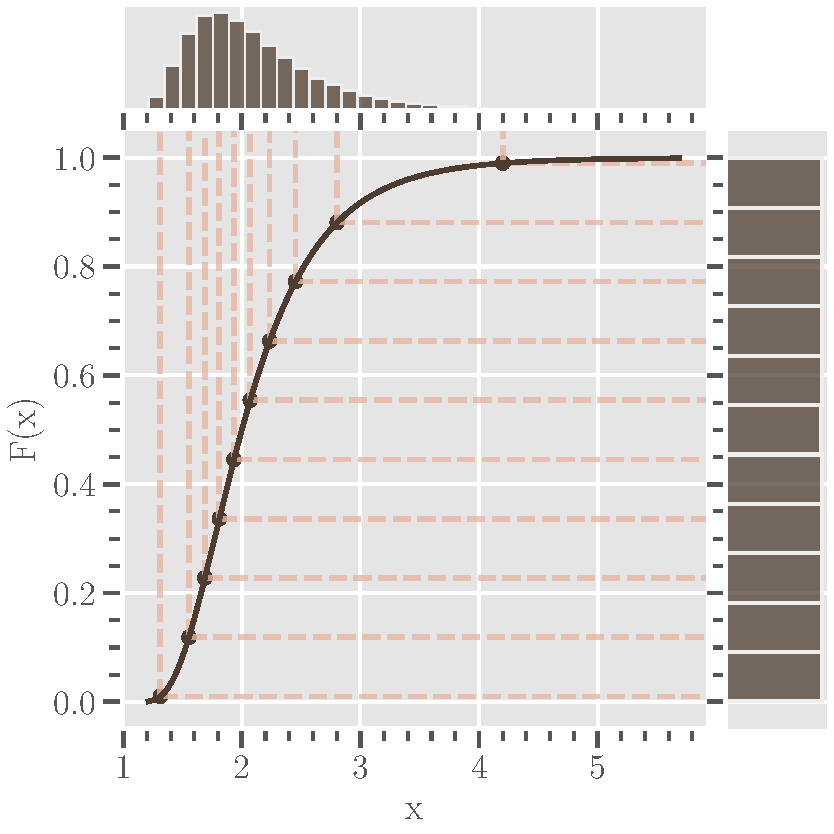
\includegraphics[width=0.6\linewidth]{01_PIT}	
	\caption{Ilustracja działania PIT. Zmienna losowa z rozkładu $
		\mathcal{LN}(0.5, 1)$ (pozioma oś) przekształcana jest przez własną dystrybuantę do rozkładu jednostajnego $\mathcal{U}(0, 1)$ (pionowa oś).\label{fig:PIT}}
\end{figure}

Wróćmy na chwilę do oryginalnego pytania, czyli modelowania wielowymiarowych zmiennych losowych. Na początku rozdziału zdefiniowaliśmy kopułę jako funkcję spełniającą równanie \ref{eq:sklar_theorem} z twierdzenia Sklara, czyli:
$$F(x_1, \dots, x_d) = C(F_1(x_1), \dots, F_d(x_d)).$$

Prawą stronę równania stanowią wyizolowane rozkłady brzegowe, oraz pewna funkcja $C$, postać której jest kompletnie od nich niezależna. Lewa strona równania, to natomiast rozkład łączny pewnej zmiennej losowej. Jeśli zastanowimy się co wpływa na charakter rozkładu łącznego zmiennej losowej, dojdziemy do wniosku, że istnieją dwa komponenty: zachowanie rozkładów brzegowych, oraz ich współzależności. Biorąc znów pod uwagę prawą stronę równania, kopuła musi więc odpowiadać za współzależności między rozkładami brzegowymi. \\
Istotnie, kopuły pozwalają na rozdzielenie problemu modelowania rozkładu łącznego, na modelowanie osobno rozkładów brzegowych, a osobno struktury ich współzależności (\cite{Sklar_Theorem}, \cite{Joe_Multivariate_Models}). Ta pozorna prostota tworzenia wielowymiarowych modeli przyczyniła się do szybkiej ich popularyzacji, ale i przyniosła ze sobą duże ryzyko modelu. Najbardziej znanym tego przykładem jest zapewne fiasko modeli wyceniających produkty typu CDO (\cite{CDS_Copula}), które niedoszacowywały nasilenia korelacji bankructw wewnątrz struktury tego kontraktu.\\

Zauważamy zatem dualizm kopuł - można patrzeć na nie zarówno jak na funkcje łączące ze sobą dowolne rozkłady brzegowe w spójny rozkład łączny, lub też jak na dystrybuanty wielowymiarowych rozkładów jednostajnych.\\
\label{subsec:dwuwymiarowe_kopuly_definicja}

\subsection{Probabilistyczna interpretacja}
Przyjrzymy się więc jednej stronie powyższego dualizmu i przeanalizujmy kopuły jako struktury zależności.

\begin{df}[Kopuła minimum]
	Dwuwymiarowa kopuła minimum $C^{-}$ to kopuła zadana wzorem $C^{-}(u, v) = \max(u+v-1, 0).$
\end{df}
\begin{df}[Kopuła maximum]
	Dwuwymiarowa kopuła maksimum $C^{+}$, to kopuła zadana wzorem $C^{+}(u, v) = \min(u, v).$
\end{df}

\begin{figure}[h]
	\centering
	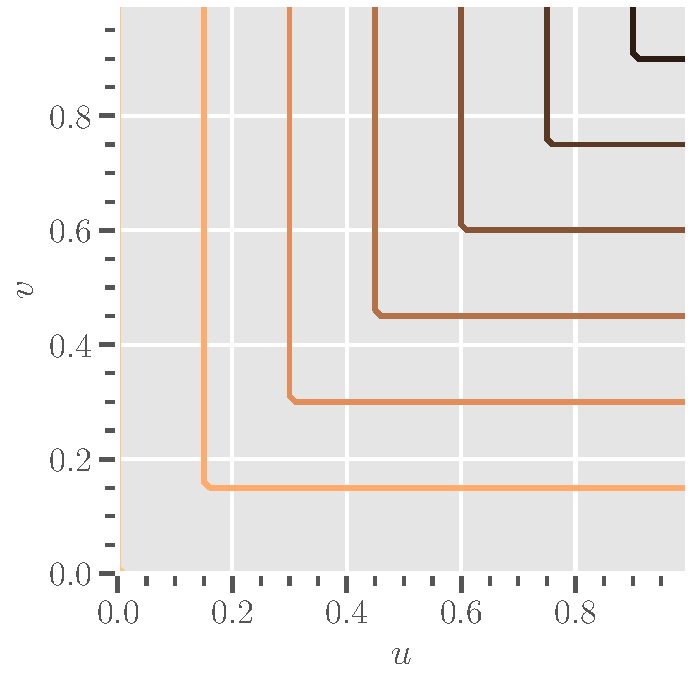
\includegraphics[width=0.35\linewidth]{01_MaximumCopula_contour}
	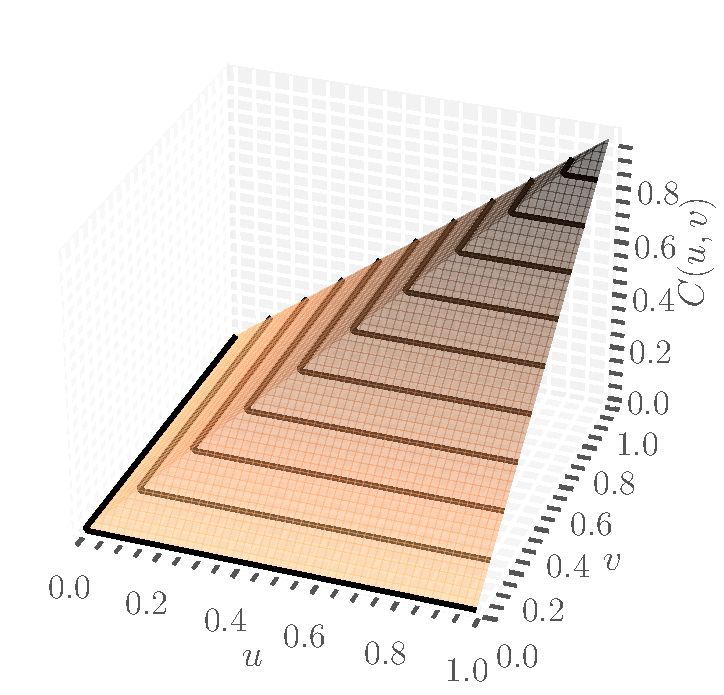
\includegraphics[width=0.4\linewidth]{01_MaximumCopula_surface}
	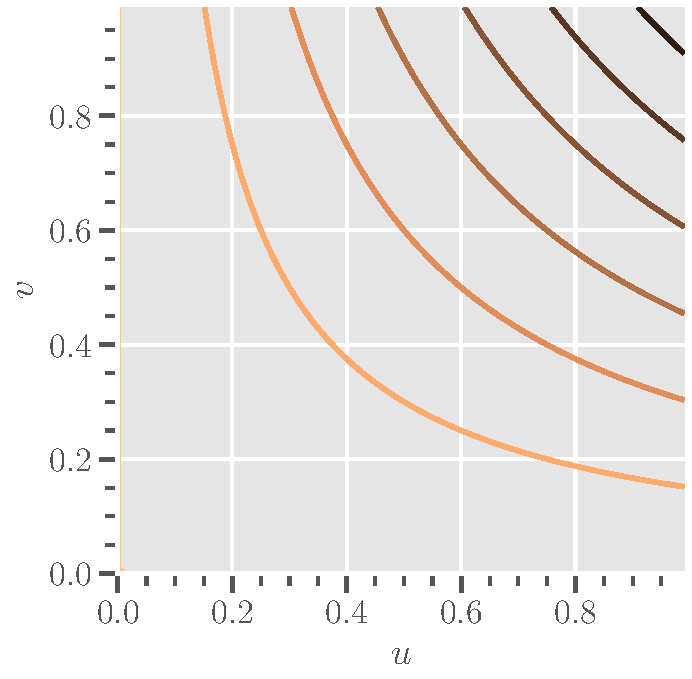
\includegraphics[width=0.35\linewidth]{01_IndependenceCopula_contour}
	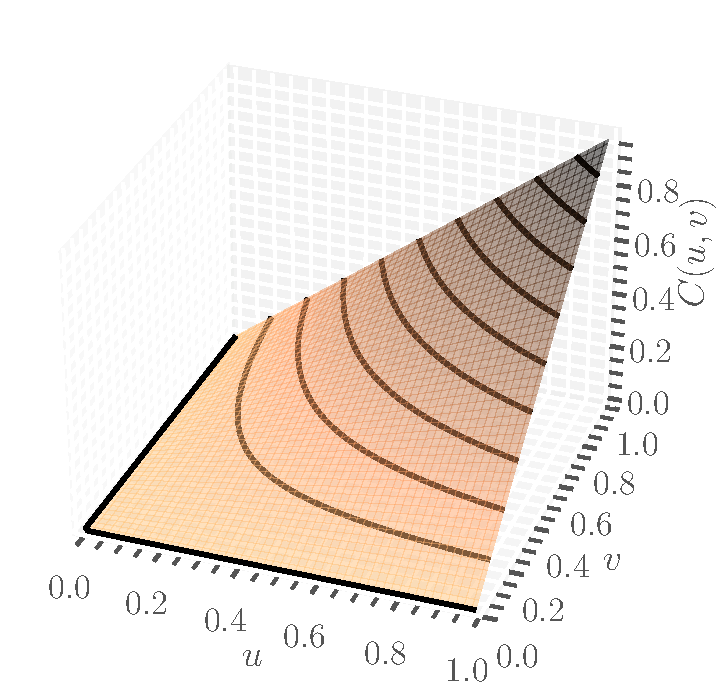
\includegraphics[width=0.4\linewidth]{01_IndependenceCopula_surface}
	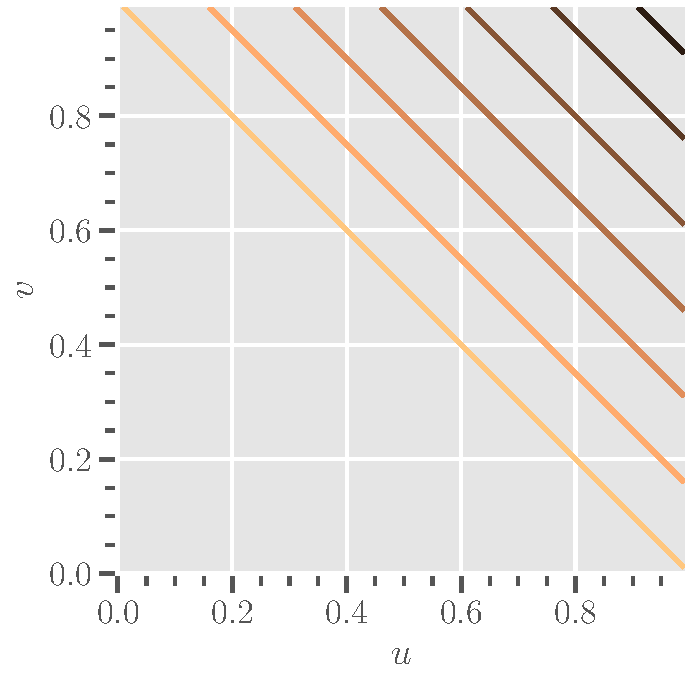
\includegraphics[width=0.35\linewidth]{01_MinimumCopula_contour}
	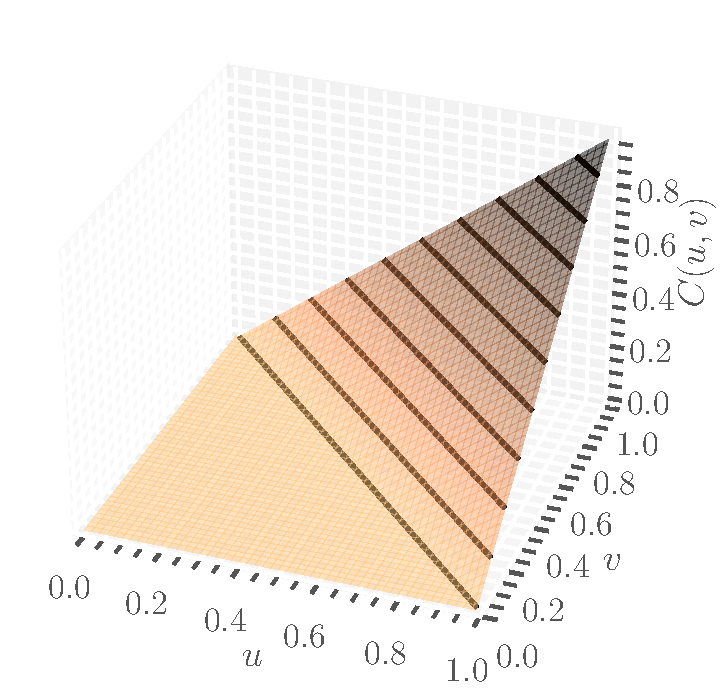
\includegraphics[width=0.4\linewidth]{01_MinimumCopula_surface}
	
	\caption{Dystrybuanty (po lewej) i kontury (po prawej) kopuł: maximum (górny panel), produktowej (panel środkowy) i minimum (dolny panel)\label{fig:minmaxprod_copula}}
\end{figure}

Powyższe kopuły stanowią horyzont osiągalnych kopuł, ponieważ jak mówi twierdzenie \ref{thm:frechet_hoeffding}, są one ograniczeniem dolnym i górnym dla dowolnej innej kopuli. Ich powierzchnie i kontury przedstawia rysunek \ref{fig:minmaxprod_copula}. 

\begin{thm}[Fréchet-Hoeffding bounds]
	Niech $C$ będzie $2$-wymiarową kopułą. Wtedy dla każdego $(u, v)\in[0, 1]^2$ zachodzi
	
	$$ C^{-}(u, v) \leqslant C(u, v) \leqslant C^{+}(u, v).$$
	
	\label{thm:frechet_hoeffding}
\end{thm}

Twierdzenie to, choć z pozoru teoretyczne, ciągnie za sobą bardzo praktyczne konsekwencje: pozwala otrzymać niezależne od modelu ogranicznia górne i dolne na dowolną kopułę. \cite{Cherubini_Copula_Methods_in_Finance} pokazuje przykład, gdzie twierdzenie Frécheta-Hoeffdinga pozwala na uzyskanie dolnego i górnego ograniczenia na pewne statystyki modelu, jak np. łączne prawdopodobieństwo bankructwa dwóch firm w strukturalnym modelu Mertona, czy cena opcji binarnej na dwa aktywa.

\begin{df}[Kopuła produktowa]
	Dwuwymiarowa kopuła produktowa $C^{\perp}$ to kopuła zadana wzorem $C^{\perp}(u, v) = uv.$
\end{df}

Kopuła produktowa jest trzecim istotnym punktem odniesienia w świecie kopuł, ponieważ posiada pewną unikalną właśność. Z jednej strony z definicji kopuły mamy:

\begin{equation}
C(u, v) = P(U \leqslant u, V \leqslant v )
\label{eq:independence_copula1}
\end{equation}

Z drugiej jednak strony, wiemy że $U$ i $V$ mają rozkłady jednostajne - więc:
\begin{equation}
	F_U(u) = P(U \leqslant u) = u\text{, oraz } F_V(v) = P(V \leqslant v) = v.
\label{eq:independence_copula2}
\end{equation}

Z równań \ref{eq:independence_copula1} i \ref{eq:independence_copula2}, dla przypadku kopuły produktowej mamy zatem:
\begin{equation}
	P(U \leqslant u, V \leqslant v ) \equiv C^{\perp}(u, v) = uv = P(U \leqslant u) P(V \leqslant v).
	\label{eq:independence_copula}
\end{equation}

Równanie \ref{eq:independence_copula} mówi nam, że zmienne losowe $V$ i $U$ są od siebie niezależne. Model kopuły produktowej, implikuje więc niezależność jednostajnych rozkładów brzegowych.
Co więcej, uzupełniając opis kopuł minimum i maksimum - te z kolei odpowiadają współmonotonicznej \emph{(eng. comonotone)} i przeciwmonotonicznej \emph{(eng. countermonotone)} zależności jednostajnych rozkładów brzegowych. Zgodnie z twierdzeniem \ref{thm:frechet_hoeffding} natomiast wszystkie inne kopuły modelują pozostałe rodzaje zależności istniejące pomiędzy tymi ekstremami. Widzimy więc, że kopuły potrafią modelować pełne spektrum możliwych zależności: od współmonotonicznych, przez niezależne, aż po przeciwmonotoniczne. 
\label{subsec:dwuwymiarowe_kopuly_probal}

\subsection{Popularne kopuły i ich własności}
Rozdział \ref{subsec:dwuwymiarowe_kopuly_probal} pokazał, że kopuły można intuicyjnie rozumieć jako modele zależności. W tej sekcji spojrzymy na nie z dualnej perspektywy, co pozwoli nam zdefiniować użyteczne narzędzia do analizy charakteru tej zależności.

\begin{df}[Gęstość kopuły]
	Niech $C$ będzie $d$-wymiarową (jednostajnie ciągłą) kopułą. Gęstością tej kopuły nazywamy funkcję
	\begin{equation}
		c(u_1, \dots, u_d) = \frac{\partial^d}{\partial u_1\dots \partial u_d}C(u_1, \dots, u_d).
		\label{eq:copula_density}
	\end{equation}
\end{df}

Widzimy, że równanie \ref{eq:copula_density} jest jedynie przeniesieniem terminu gęstości rozkładu na grunt kopuł. Zanim zaczniemy wizualizować gęstości konkretnych kopuł, warto wspomnieć, że Sklar w \cite{Sklar_Theorem} podaje również alternatywną wersję swojego twierdzenia o istnieniu kopuły, tym razem w języku gęstości. Sens i zastosowania twierdzenia pozostają takie same jak przy \ref{thm:sklar_theorem}.
\begin{thm}[Twierdzenie Sklara: gęstość kopuły]
	Niech $X$ będzie $d$-wymiarowym wektorem losowym o dystrybuancie rozkładu łącznego $F$, oraz rozkładami brzegowymi $F_i$, $i=1, \dots, d$. Wtedy rozkład łączny może być wyrażony jako		$$F(x_1, \dots, x_d) = C(F_1(x_1), \dots, F_d(x_d)),$$
	lub równoważnie w terminach gęstości poprzez:
	$$ f(x_1, \dots, x_d) = c(F_1(x_1), \dots, F_d(x_d))\cdot f_1(x_1)\dots f_d(x_d),$$
	dla pewnej $d$-wymiarowej kopuli $C$, o gęstości $c$. Dla rozkładów bezwzględnie ciągłych, kopuła $C$ jest jednoznacznie określona.\\
	Zachodzi również twierdzenie odwrotne: kopuła związana z wielowymiarowym rozkładem $F$ o rozkładach brzegowych $F_1, \dots F_d$ może być wyrażona jako:
	$$C(u_1, \dots, u_d) = F(F_1^{-1}(u_1), \dots, F_d^{-1}(u_d)),$$
	a jej gęstość wyraża się poprzez:
	$$c(u_1, \dots, u_d) = \frac{f(F_1^{-1}(u_1), \dots, F_d^{-1}(u_d))}{f_1(F_1^{-1}(u_1))\dots f_d(F_d^{-1}(u_d))}$$
	\label{thm:sklar_theorem_density}
\end{thm}

Resztę rozdziału stanowić będzie opis rodzin kopuł o istotnych zastosowaniach w praktyce.\\

\underline{Kopuła produktowa}\\

Gęstość kopuły produktowej otrzymujemy różniczkując jej dystrybuantę:
$$ c(u, v) =\frac{\partial^2}{\partial u\partial v}C(u, v) = 1. $$ 

\begin{figure}[h]
	\centering
	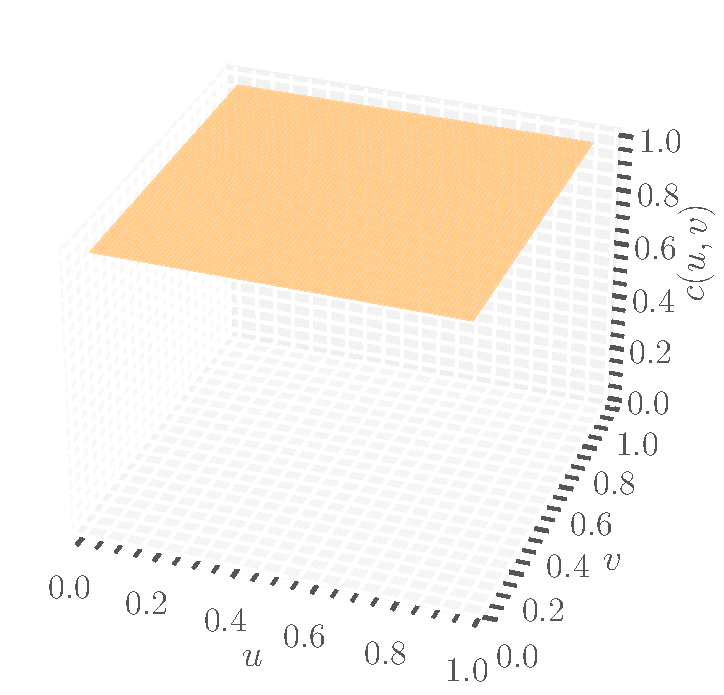
\includegraphics[width=0.4\linewidth]{01_IndependenceCopula_density}
	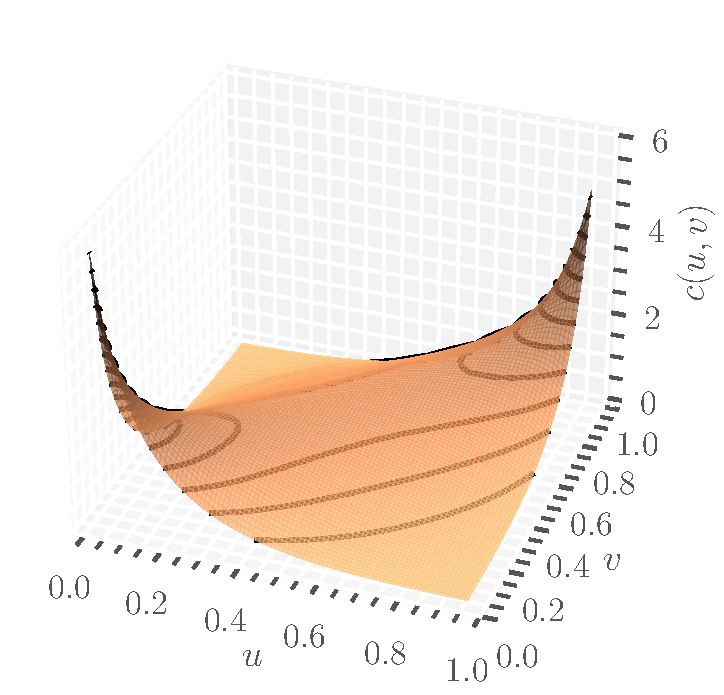
\includegraphics[width=0.4\linewidth]{01_GaussianCopula_density}
	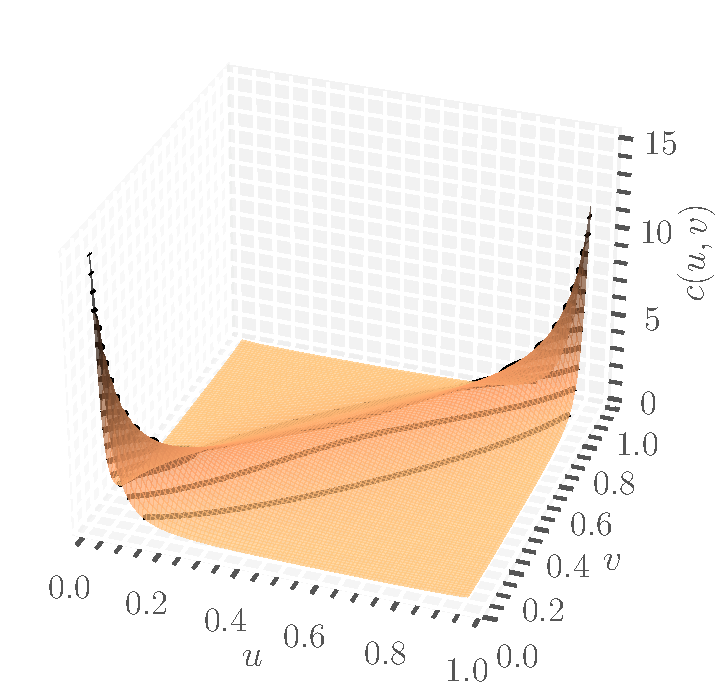
\includegraphics[width=0.4\linewidth]{01_StudentCopula_density}
	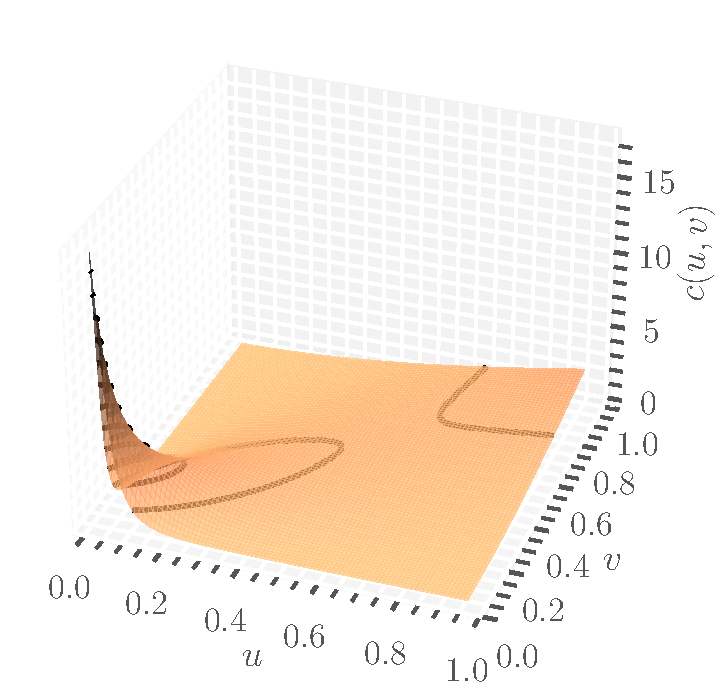
\includegraphics[width=0.4\linewidth]{01_ClaytonCopula_density}
	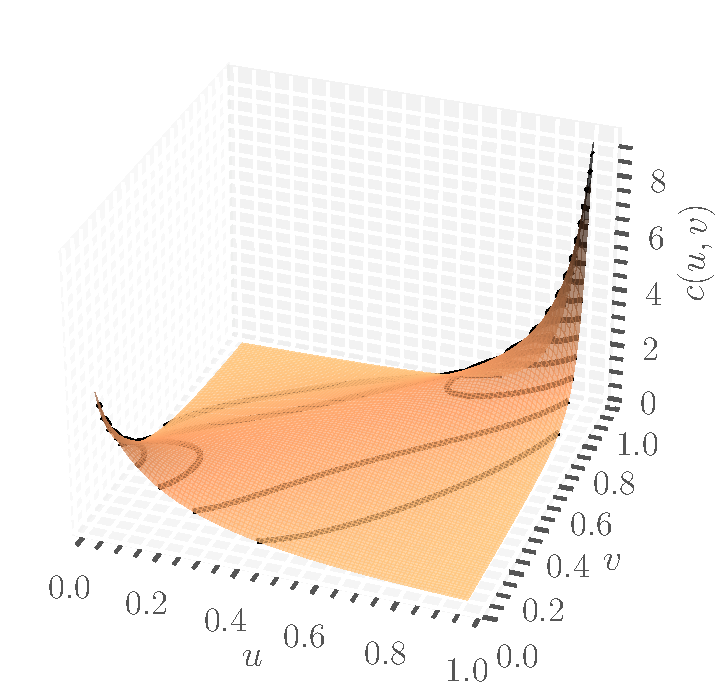
\includegraphics[width=0.4\linewidth]{01_GumbelCopula_density}
	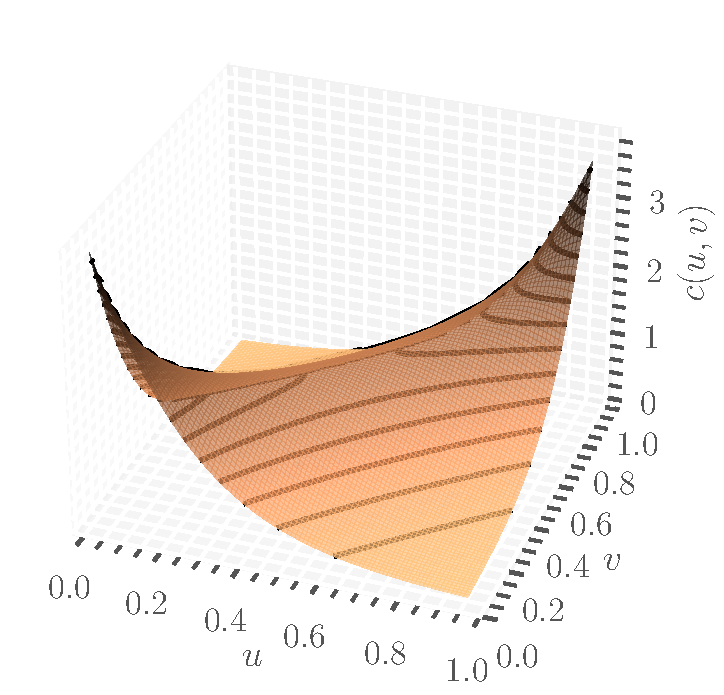
\includegraphics[width=0.4\linewidth]{01_FrankCopula_density}
	
	\caption{Gęstości wybranych kopuł.\label{fig:copula_densities}}
\end{figure}

\label{subsec:dwuwymiarowe_kopuly_przyklady}



\section{Vine Copulas}
\label{sec:vine_copulas}
Problemy z którymi spotykamy się w praktyce są nierzadko z natury wielowymiarowe. W rozdziale \ref{sec:popularne_spready} opowiemy o clean dark spreadach, czyli mierze rentowności elektrowni węglowej który wymaga modelowania zależności trzech komponentów (ceny węgla, ceny certyfikatów emisyjnych i ceny energii). Model LDA dla ryzyka operacyjnego nadmieniony w rozdziale \ref{subsec:dwuwymiarowe_kopuly_przyklady} wymaga segmentacji strat względem przynależności do jednej z kilkunastu/kilkudziesięciu homogenicznych kategorii (ORC) i modelowania zależności między nimi. Natomiast modelowanie zależności komponentów portfela inwestycyjnego może okazać się nawet kilkusetwymiarowym problemem.\\
Widzimy więc, że przekrój zastosowań praktycznych jest bardzo duży i istnieje zapotrzebowanie na wielowymiarowe modele zależności. Dwuwymiarowe kopuły przedstawione w \ref{subsec:dwuwymiarowe_kopuly_przyklady} mają często swoje wielowymiarowe odpowiedniki (\cite{Cherubini_Copula_Methods_in_Finance}, \cite{Kurowicka_Dependence_Modeling}). Są one jednak stosunkowo mało elastyczne, ponieważ nie pozwalają ,,dostroić" modelu na poziomie interakcji każdej pary wymiarów zmiennej losowej. W tym rozdziale sięgniemy po modele Vine Copula, które pozwolą modelować wielowymiarowe zależności w dużych detalach, do stopnia gdzie będziemy w stanie określić zależność między dowolnymi dwoma rozkładami brzegowymi.\\

\subsection{Pair Copula Constructions}
\label{subsec:pair_copula_constructions}
Zaczniemy od przykładu w trzech wymiarach, aby zilustrować czym jest \emph{Pair copula construction} (PCC). Ogólną ideą jest aby wielowymiarowy rozkład zmiennej losowej rozbić na dwuwymiarowe komponenty modelowane za pomocą dwuwymiarowych kopuł.\\

W poniższych rozważaniach przydadzą nam się następujący lemat dotyczący relacji między gęstością kopuły a rozkładami warunkowymi:

\begin{lemma}
	Rozkład warunkowy dwuwymiarowej zmiennej losowej można przedstawić w języku kopuły:	
	$$ f_{1|2}(x_1|x_2) =c_{12}(F_1(x_1), F_2(x_2))f_2(x_2).$$
	\label{lem:copula_representation_of_conditional_density}
\end{lemma}
\begin{proof}
	Posługując się twierdzeniem Sklara \ref{thm:sklar_theorem_density} mamy:
	\begin{equation*}
		\begin{split}
			f_{1|2}(x_1, x_2) & = \frac{f_{12}(x_1, x_2)}{f_2(x_2)} \\
			& = \frac{c_{12}(F_1(x_1), F_2(x_2))f_1(x_1)f_2(x_2)}{f_2(x_2)}\\
			& = c_{12}(F_1(x_1), F_2(x_2))f_1(x_1)
		\end{split}
	\end{equation*}
\end{proof}

\subsubsection{Przykład ilustrujący}
\label{subsub:przyklad_3_wymiary}
Aby zilustrować PCC, rozpatrzmy rozkład $3$-wymiarowy o gęstości $f(x_1, x_2, x_3)$. Tę gęstość można przedstawić w postaci:

$$ f(x_1, x_2, x_3) = f_{3|12}(x_3|x_1, x_2)f_{2|1}(x_2|x_1)f_1(x_1).$$

Celem jest sfaktoryzowanie tego wyrażenia do postaci wykorzystującej co najwyżej dwuwymiarowe kopuły lub jednowymiarowe rozkłady brzegowe. Widzimy, że w tym celu należy rozwinąć $f_{3|12}$ oraz $f_{2|1}$. \\
Korzystając z lematu \ref{lem:copula_representation_of_conditional_density} otrzymujemy bezpośrednio $f_{2|1}$ oraz $f_{3|1}$ (które przyda się za chwilę) jako:
\begin{equation*}
	\begin{split}
		f_{1|2}(x_1|x_2) &= c_{12}(F_1(x_1), F_2(x_2))f_2(x_2),\\
		f_{3|2}(x_3|x_2) &= c_{32}(F_3(x_3), F_2(x_2))f_2(x_2)
	\end{split}
\end{equation*}

Natomiast w celu otrzymania $f_{3|12}$ będziemy musieli przejść przez dwuwymiarowy rozkład $f_{13|2}(x_1, x_3|x_2)$. Ma on rozkłady brzegowe $F_{1|2}(x_1|x_2)$ oraz $F_{3|2}(x_3|x_2)$ i kopułę warunkową $c_{13;2}$~-~czyli kopułę rozkładu $(X_1, X_3) | X_2=x_2$. Zaaplikujemy do niego twierdzenie Sklara \ref{thm:sklar_theorem_density}:

\begin{equation*}
	\begin{split}
		f_{3|12}(x_3|x_1,x_2)  & = \frac{f_{13|2}(x_1, x_3|x_2)}{f_{1|2}(x_1|x_2)} \\
		& = \frac{c_{13;2}(F_{1|2}(x_1|x_2), F_{3|2}(x_3|x_2); x_2)f_{1|2}(x_1|x_2)f_{3|2}(x_3|x_2)}{f_{1|2}(x_1|x_2)}\\
		& = c_{13;2}(F_{1|2}(x_1|x_2), F_{3|2}(x_3|x_2); x_2)f_{3|2}(x_3|x_2) \\
		& = c_{13;2}(F_{1|2}(x_1|x_2), F_{3|2}(x_3|x_2); x_2)c_{32}(F_3(x_3), F_2(x_2))f_2(x_2)
	\end{split}
\end{equation*}

Finalnie otrzymujemy dekompozycję $f(x_1, x_2, x_3)$ do postaci:

\begin{equation}
	\begin{split}
	f(x_1, x_2, x_3) = &c_{13;2}(F_{1|2}(x_1|x_2), F_{3|2}(x_3|x_2); x_2) \cdot \\
	& c_{23}(F_2(x_2), F_3(x_3)) \cdot c_{12}(F_1(x_1), F_2(x_2)) \cdot \\
	& f_3(x_3)f_2(x_2)f_1(x_1).
	\end{split}
	\label{eq:PCC}
\end{equation}

Powyższe czynniki są jedynie dwuwymiarowymi kopułami oraz rozkładami warunkowymi lub brzegowymi. Taką dekompozycję nazwiemy Pair Copula Construction (PCC). Zaletą takiej reprezentacji nad wielowymiarową kopułą jest to, że ma większą liczbę niżej-wymiarowych komponentów, przez co pozwala lepiej dopasować model do danych. Realne dane rzadko mają regularną strukturę zależności która może być dobrze opisana jedną, wielowymiarową kopułą (\cite{Czado_Vine_Copulas}), dlatego też PCC radzi sobie z tym lepiej.\\
Zwróćmy jednak uwagę na fakt, że nie jest to jedyna PCC która opisuje rozkład $f(x_1, x_2, x_3)$. Istnieją poniższe, równoważne reprezentacje - do których wrócimy pod koniec sekcji \ref{subsec:vine_copula}.

\begin{equation}
	\begin{split}
		f(x_1, x_2, x_3) = &c_{12;3}(F_{1|3}(x_1|x_3), F_{2|3}(x_2|x_3); x_3) \cdot \\
		& c_{13}(F_1(x_1), F_3(x_3)) \cdot c_{23}(F_2(x_2), F_3(x_3)) \cdot \\
		& f_3(x_3)f_2(x_2)f_1(x_1).
	\end{split}
\end{equation}

\begin{equation*}
	\begin{split}
		f(x_1, x_2, x_3) = &c_{23;1}(F_{2|1}(x_2|x_1), F_{3|1}(x_3|x_1); x_1) \cdot \\
		& c_{13}(F_1(x_1), F_3(x_3)) \cdot c_{12}(F_1(x_1), F_2(x_2)) \cdot \\
		& f_3(x_3)f_2(x_2)f_1(x_1).
	\end{split}
\end{equation*}
	
\subsection{Vine Copula}
\label{subsec:vine_copula}
Ideę rozbijania rozkładu na dwuwymiarowe bloki da się rozszerzyć na $d$-wymiarów. Podobnie jednak jak w przykładzie 3-wymiarowym z sekcji \ref{subsub:przyklad_3_wymiary}, nie mamy jedyności tej reprezentacji - istnieje wiele różnych dróg do osiągnięcia tego samego celu. 

\begin{thm}[$d$-wymiarowa PCC]
	Niech $f_{1,2,\dots,d}$ będzie gęstością łączną $d$-wymiarowego rozkładu. Możemy ją wyrazić poprzez:
	
	\begin{equation}
		f_{1,\dots, d}(x_1, \dots, x_d) = \bigg[ \prod_{j=1}^{d-1} \prod_{i=1}^{d-j} c_{i, (i+j); (i+1)\dots(i+j-1)} \bigg] \cdot \bigg[ \prod_{k=1}^{d}f_k(x_k)\bigg].
		\label{eq:recursive_pcc}
	\end{equation}
\end{thm}
\begin{proof}
	Zacznijmy od rozważenia rozkładu łącznego i jego ogólnej rekursywnej dekompozycji:
\begin{equation}
	\begin{split}
		f_{1, \dots, d}(x_1, \dots, x_d) &= f_{d|1 , \dots, d-1}(x_d|x_1, \dots, x_{d-1})f_{1,\dots,d-1}(x_1, \dots, x_{d-1})\\
		&=\dots= \bigg[\prod_{t=2}^{d}f_{t|1,\dots,t-1}(x_t|x_1, \dots, x_{t-1})\bigg]\cdot f_1(x_1)
	\end{split}
	\label{eq:d-dimensional_decomp}
\end{equation}

Teraz użyjemy lematu \ref{lem:copula_representation_of_conditional_density} do rozkładu warunkowego $(X_1, X_t) | (X_2, \dots, X_{t-1})$ żeby wyrazić $f_{t|1,\dots,t-1}(x_t|x_1,\dots,x_{t-1})$.
	\begin{equation}
	\begin{split}
	f_{t|1,\dots,t-1}(x_t|x_1,\dots,x_{t-1})&= c_{1,t|2,\dots,t-1}\cdot f_{t|2,\dots,t-1}(x_t|x_2,\dots,x_{t-1})  \\
	& = \bigg[ \prod_{s=1}^{t-2} c_{s,t;s+1,\dots,t-1} \bigg] c_{(t-1), t} f_t(x_t).	
	\end{split}
	\end{equation}

Aplikując \ref{eq:recursive_pcc} do równania \ref{eq:d-dimensional_decomp}, oraz oznaczając $s=i, t=i+j$ możemy zapisać:

\begin{equation*}
	\begin{split}
		f_{1, \dots, d}(x_1, \dots, x_d) &= \bigg[\prod_{t=2}^{d}\prod_{s=1}^{t-2} c_{s,t;s+1,\dots,t-1}\bigg] \cdot \bigg[ \prod_{t=2}^{d}c_{(t-1), t} \bigg] \cdot \bigg[ \prod_{k=1}^{d}f_{k}(x_k) \bigg] = \\
		& = \bigg[\prod_{j=1}^{d-1}\prod_{i=1}^{d-j}c_{i,(i+j);(i+1)\dots(i+j-1)}\ \bigg] \cdot \bigg[\prod_{k=1}^{d}f_k(x_k)\bigg].
	\end{split}
\end{equation*}
\end{proof}

Jak widać z równania \ref{eq:d-dimensional_decomp}, dekompozycje te potrafią być zawiłe i mało interpretowalne. Do tego dochodzi fakt, że podobnie jak w przykładzie 3-wymiarowym, nie jest to jedyna postać dekompozycji. Dlatego wprowadzimy teraz fragmenty teorii grafów, która pozwoli nam lepiej komunikować i zrozumieć strukturę PCC.

\begin{df}[Graf, wierzchołek, krawędź, stopień]
	Grafem nazwiemy parę zbiorów $G= (N, E)$, takich że $E \subseteq \{ \{x,y \}: x,y \in N \}$.
	\begin{itemize}
		\item Elementy $E$ nazywać będziemy krawędziami grafu $G$, a elementy $N$ wierzchołkami
		\item Liczbę sąsiadów wierzchołka $v\in N$ będziemy nazywać jego stopniem i oznaczać $d(v)$
	\end{itemize}
\end{df}

\begin{df}[Ścieżka, cykl, graf spójny, graf acykliczny]
	Ścieżka to rodzaj grafu $P = (N, E)$ o wierzchołkach $N = \{ v_0, v_1, \dots, v_k\}$ i krawędziach \\ $E = \{ \{v_0, v_1 \}, \{v_1, v_2 \}, \{v_2, v_3 \}, \dots, \{v_{k-1}, v_k \} \}$.\\
	Cyklem nazywamy ścieżkę gdzie $v_0=v_k$.\\
	Jeżeli dla każdej pary wierzchołków istnieje łącząca je ścieżka, to graf nazwiemy spójnym. Jeżeli graf nie zawiera w sobie cykli, to nazwiemy go acyklicznym. 
\end{df}

\begin{figure}[h]
	\centering
	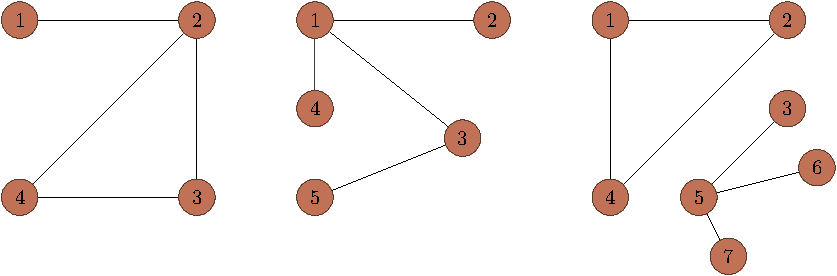
\includegraphics[width=\linewidth]{03_example_graph}
	
	\caption{\textbf{Przykłady grafów.} Cykliczny spójny (po lewej), acykliczny spójny (na środku), cykliczny niespójny (po prawej)\label{fig:example_graph}}
\end{figure}

Przykładowe grafy przedstawione sa na rysunku \ref{fig:example_graph}. Nas interesować będą jednak szczególne rodzaje grafów, nazywane drzewami.
\begin{df}[Charakteryzacja drzewa]
	Poniższe stwierdzenia są równoważne dla grafu $T = (N, E)$:
	\begin{enumerate}
		\item $T$ jest drzewem
		\item Dowolne dwa węzły grafu $T$ są połączone unikalną ścieżką w $T$.
		\item $T$ jest grafem spójnym, ale $T-e$ jest niespójnym dla dowolnej krawędzi $e\in E$
		\item $T$ jest grafem acyklicznym, ale $T +\{x,y\}$ będzie zawierać cykl dla dowolnych dwóch niesąsiadujących wierzchołków $x, y \in N$.
	\end{enumerate}
\end{df}

Jedynym drzewem widocznym na rysunku \ref{fig:example_graph} jest graf na środkowym panelu. Drzewa są istotne w teorii wielowymiarowych kopuł, ponieważ stanowią podstawowy element budujący \emph{regular vines}, czyli zbiory grafów które posłużą nam do przedstawiania struktury PCC.

\begin{df}[Regular vine]
	Zbiór drzew $\Nu = (T_1,\dots, T_{d-1})$ nazywamy \emph{regular vine}, lub \emph{R-vine} jeżeli:
	
	\begin{enumerate}
		\item Każde drzewo $T_j=(N_j, E_j)$ jest spójne
		\item $T_1$ jest drzewem o zbiorze wierzchołków $N_1$ i zbiorze krawędzi $E_1$
		\item Dla $j\geqslant2$, $T_j$ jest drzewem o zbiorze wierzchołków $N_j = E_{j-1}$ i zbiorze krawędzi $E_{j-1}$
		\item Dla $j = 2, \dots, d- 1$ oraz $\{a, b\} \in E_j$ mamy $ \vert a \cap b \vert = 1$. 
	\end{enumerate}
\end{df}

Na wykresie \ref{fig:r_vine} pokazujemy przykładową strukture R-vine. Opisu krawędzi i wierzchołków dokonujemy zgodnie z wprowadzanym poniżej pojęciem warunkowego i warunkowanego zbioru.

\begin{df}[Zbiór warunkowy, zbiór warunkowany]
	Dla dowolnej krawędzi $e\in E_i$ zdefiniujmy zbiór:
	$$ A_e\coloneqq \{j\in N_1\vert \exists e_1 \in E_1, \dots, e_{i-1}\in E_{i-1}: j\in e_1\in \dots \in e_{i-1}\in e\}.$$
	Zbiorem warunkującym $D_e$ krawędzi $e=\{a, b\}$ nazywamy:
	
	$$ D_e \coloneqq A_a \cup A_b,$$
	
	zbiorami warunkowanymi $C_{e, a}$ i $C_{e, b}$ nazywamy natomiast:
	
	$$ C_{e, a} \coloneqq A_a\\ D_e$$
	$$ C_{e, b} \coloneqq A_b\\ D_e.$$
	
	Skrótowo, będziemy opisywać krawędź $e = (C_{e, a}, C_{e, b}; D_e)$ jako $e = (e_a, e_b; D_e)$.
\end{df}


\begin{figure}[h]
	\centering
	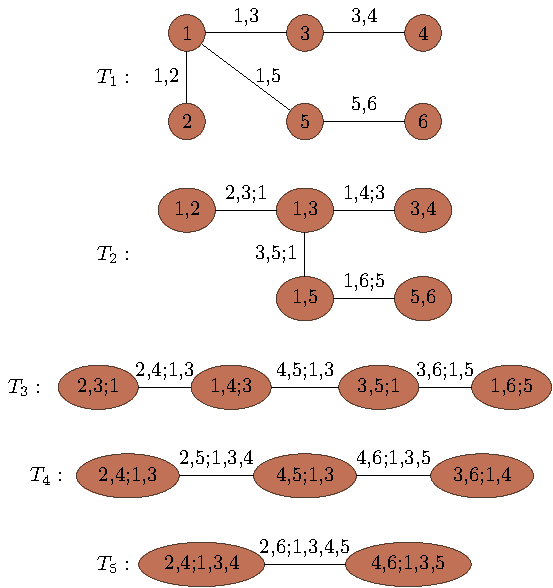
\includegraphics[width=0.7\linewidth]{03_R_vine}
	
	\caption{\textbf{Regular vine}. Przykładowa 6-wymiarowa struktura R-vine. \label{fig:r_vine}}
\end{figure}

Definicja struktury R-vine nie narzuca szczególnej postaci drzew. Jeżeli zaczniemy stawiać pewne warunki na ich strukturę, to trafimy w szczególności w dwie podklasy: D-vine i C-vine (rysunek \ref{fig:d_vine_c_vine}). D-vine zachodzi gdy każdy wierzchołek ma stopień co najwyżej równy dwa - powoduje to że drzewa wyglądają jak łańcuchy i nie mają odgałęzień. C-vine natomiast pojawia się w przypadku gdy każde drzewo ma pewien \emph{root node}, który jest połączony z każdym innym wierzchołkiem.
\begin{df}[D-vine, C-vine]
	Niech $\Nu$ będzie strukturą R-vine.
	\begin{enumerate}
		\item Jeżeli dla każdego wierzchołka $n\in N_i$ zachodzi warunek $\vert \{e\in E_i\vert n\in e\}\vert \leqslant 2$, to należy ona do podklasy \emph{D-vine} (drawable vine).
		\item Jeżeli dla każdego drzewa $T_i$ istnieje wierzchołek $n\in N_i$ taki, że $\vert \{e\in E_i\vert n\in e\}\vert = d-i$, to należy ona do podklasy \emph{C-vine} (canonical vine).
	\end{enumerate}
\end{df}


\begin{figure}[h]
	\centering
	\begin{minipage}{0.35\linewidth}
	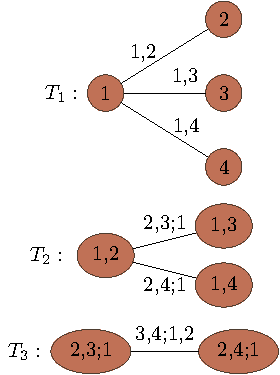
\includegraphics[width=\linewidth]{03_C_vine}
	\end{minipage}	
	\begin{minipage}{0.45\linewidth}
	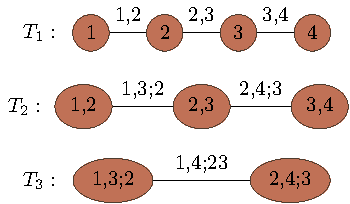
\includegraphics[width=\linewidth]{03_D_vine}
	\end{minipage}	

	\caption{\textbf{Canonical vine i Drawable vine.} Przykładowa 4-wymiarowa struktura C-vine (lewy panel) i D-vine (prawy panel).\label{fig:d_vine_c_vine}}
\end{figure}

Struktury R-vine są przydatne do wyjaśniania struktury zależności wielowymiarowych rozkładów, ponieważ jak pokazali \cite{BedfordCooke2002}, istnieje połączenie między PCC a pewnym R-vine.

\begin{df}[Rozkłady R-vine]
	Mówimy, że rozkład $F$ dla $d$-wymiarowego wektora losowego $(X_1, \dots, X_d)$ jest \emph{rozkładem R-vine}, jeśli możemy podać trójkę $(\mathcal{F}, \Nu, \mathcal{B})$ o własnościach:
	\begin{itemize}
		\item $\mathcal{F} =(F_1, \dots, F_d)$ jest wektorem ciągłych, odwracalnych dystrybuant rozkładów brzegowych $(X_1, \dots, X_d)$
		\item $\Nu$ jest $d$-wymiarową strukturą R-vine 
		\item Zbiór $\mathcal{B} = \{C_e\vert e \in E_i; i=1,\dots,d-1\}$, gdzie $C_e$ jest radialnie symetryczną dwuwymiarową kopułą posiadającą gęstość.
		\item Dla każdego $e\in E_i, i=1, \dots, d-1, e=\{a,b\}$, $C_e$ jest kopułą związaną z rozkładem warunkowym $X_{C_{e, a}}, X_{C_{e, b}}$ pod warunkiem $X_{D_e} = x_{D_e}$.
	\end{itemize}
	\label{def:r_vine_distribution}
\end{df}

W swojej pracy, Bedford i Cooke pokazują w szczególności, że dowolną trójkę $(\mathcal{F}, \Nu, \mathcal{B})$ o własnościach z definicji \ref{def:r_vine_distribution} można związać z pewnym $d$-wymiarowym rozkładem $F$.

\begin{thm}[Istnienie rozkładu R-vine]
	Niech $(\mathcal{F}, \Nu, \mathcal{B})$ spełnia warunki z definicji \ref{def:r_vine_distribution}. Wtedy istnieje dokładnie jeden $d$-wymiarowy rozkład $F$ o gęstości:
	
	\begin{equation*}
		\begin{split}
			f_{1, \dots, d}(x_1, \dots, x_d) = &f_1(x_1)\dots f_d(x_d) \cdot\\
			& \cdot \prod_{i=1}^{d-1}\prod_{e\in E_i}c_{C_{e, a}C_{e, b};D_e}(F_{C_{e, a}\vert D_e}(x_{C_{e, a}|x_{D_e}}), F_{C_{e, b}\vert D_e}(x_{C_{e, b}|x_{D_e}})),
		\end{split}
	\end{equation*}

	taki, że dla każdego $e\in E_i, i = 1,\dots, d-1$ oraz $e=\{a, b\}$ rozkład $X_{C_{e, a}}$ i $X_{C_{e,b}}$ pod warunkiem $X_{D_e} = x_{D_e}$ wyraża się poprzez:
	
	$$ F_{C_{e, a}C_{e, b}\vert D_e}(x_{C_{e, a}}, x_{C_{e, b}}|x_{D_e}) = C_{e}(F_{C_{e, a}\vert D_e}(x_{C_{e, a}|x_{D_e}}), F_{C_{e, b}\vert D_e}(x_{C_{e, b}|x_{D_e}})).$$
	
	Ponadto rozkłady brzegowe $F$ zadane są jako $F_i(x_i), i = 1,\dots, d.$
	\label{thm:existence_of_r_vine}
\end{thm}

Warunki z twierdzenia \ref{def:r_vine_distribution}, nie są znacząco restrykcyjne - jedynym potencjalnie problematycznym założeniem jest tu ciągłość rozkładów brzegowych i odwracalność dystrybuant. W praktyce więc można korzystać z wyniku \ref{thm:existence_of_r_vine} aby związać wielowymiarowy rozkład z reprezentacją R-vine.\\
Z twierdzenia \ref{thm:existence_of_r_vine} wynika nie tylko istnienie rozkładu R-vine, ale i również to, że dekompozycja używa kopuł związanych ze zbiorami warunkowymi obecnymi na grafie struktury R-vine i \emph{vice versa}. Z każdym wierzchołkiem i krawędzią struktury można więc związać pewien element dekompozycji - dwuwymiarową kopułę lub rozkład brzegowy. Wracając do przykładu z rozdziału \ref{subsub:przyklad_3_wymiary}, gdzie dla 3-wymiarowego rozkładu dostepne były trzy dekompozycje, możemy teraz zwizualizować te możliwości poprzez użycie struktury D-vine. Na rysunku \ref{fig:PCCs} widać, że dekompozycja zalezy jedynie od kolejności wymiarów w drzewie $T_1$.

\begin{figure}[h]
	\centering
	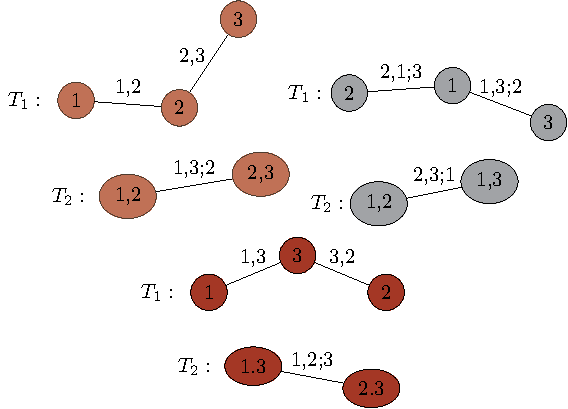
\includegraphics[width=0.8\linewidth]{03_PCC}
	
	\caption{\textbf{Pair Copula Constructions.} Trzy możliwe dekompozycje PCC 3-wymiarowego rozkładu, przedstawione w postaci R-vine. \label{fig:PCCs}}
\end{figure}

Widzimy zatem, że Vine Copula są przydatnym narzędziem pozwalającym na tworzenie bardzo elastycznych modeli, mających na celu lepsze, bardziej skrojone na wymiar uchwycenie struktury zależności w danych.\\
W kolejnym rozdziale opiszemy finansowe \emph{spready} będące funkcją ceny kilku aktywów rynkowych. Zaprezentujemy kilka sposobów na ich modelowanie, i pokażemy bardzo generalną metodę wykorzystującą Vine Copulas.

		
\mgrclosechapter
\chapter{Spready na rynkach finansowych}
Według prognoz \cite{PetroleumForecasts} z sierpnia 2022 roku, średnie zapotrzebowanie na paliwa w całym 2022 wyniesie $99.4$ milionów baryłek ropy dziennie. Ta średnia jest o $2.1$ miliona baryłek wyższa niż w roku 2021. Koncerny naftowe przerabiające na dużą skalę ropę na produkty ropopochodne muszą więc obracać gigantyczną ilością towaru, którego cena fluktuuje każdego dnia.
Niezależnie od woli koncernu zmienia się nie tylko cena nabywanej ropy ale i cena sprzedawanego paliwa. Na ich zyski, oprócz długiej listy kosztów operacyjnych wpływa naturalnie różnicą pomiędzy ceną sprzedaży produktu, a ceną zakupu surowca. Różnica ta jest przykładem \emph{processing spreadu}, który jest źródłem ryzyka rynkowego dla producenta dowolnego towaru. Jeśli spread niebezpiecznie się zawęża, producent tracić będzie zyski, a przy pewnej krytycznej wartości zmuszony wręcz będzie wstrzymać produkcję. Uczestnicy rynku świadomi ryzyka, mogą użyć instrumentów pochodnych na spread w celu zagwarantowania ciągłości produkcji nawet w wypadku niekorzystnych warunków rynkowych (\cite{KGHM}). W szczególności na rynku surowców, używanie kontraktów futures czy opcji na spread jest popularną metodą zabezpieczania się przed ryzykiem rynkowym (\cite{spread_hedging}).

W tym rozdziale opiszemy popularne rodzaje spreadów, odwołamy się do popularnych modeli pozwalających wyceniać instrumenty pochodne na spread, oraz w szczególności omówimy model bazujący na dwuwymiarowych kopułach.


\section{Popularne rodzaje spreadów}
Rynki finansowe pełne są przykładów spreadów pomiędzy różnymi aktywami. Od spreadów między stopami procentowymi, po różnorakie spready na rynkach energii, wiele z nich wykształciło swoją pozycję jako samoistne aktywa, nierzadko z płynnym rynkiem na instrumenty pochodne \cite{Carmona_Spread_Options}.\\
Poniżej wymienimy różne rodzaje spreadów z wybranych rynków, aby dać czytelnikowi ideę o ich różnorodnej naturze. Jednak w obliczu mnogości rodzajów spreadów, tej listy w żaden sposób nie można nazwać wyczerpującą.\\

Spreadem nazywać będziemy różnicę pomiędzy cenami dwóch aktywów $S_1$ i $S_2$:
$$ s(t) = S_1(t) - S_2(t).$$
Jest to najprostsza wersja spreadu, jaką jest np. \emph{bid-ask} spread, czyli różnica między ceną kupna a sprzedaży aktywa na giełdzie. Definicję tę rozszerzać można jednak do liniowych kombinacji, oraz do większej liczby aktywów - co w praktyce jest nieuniknione (ze względu na różne jednostki komponentów spreadu, lub większą ilość komponentów) więc w pełnej ogólności rozważać będziemy:
$$ s(t) = \alpha_1S_1(t) - \alpha_2S_2(t) - \cdots -\alpha_nS_n(t).$$

\subsubsection{Rynek instrumentów o stałym dochodzie}

Rynek instrumentów o stałym dochodzie posiada bogatą gamę spreadów. Spread między stopami swapowymi różnych krajów, mierzy (implikowane) różnice pomiędzy tymi rynkami dotyczące ryzyka kredytowego i ryzyka płynności. Przykładami mogą być spready francusko-niemieckie, czy niemiecko-duńskie. Inną klasą spreadów na tym rynku jest spread kredytowy - czyli różnica między stopą zwrotu obligacji obarczonych ryzykiem, jak korporacyjne, względem zwrotu z obligacji o znikomym ryzyku, jak rządowe. Jest to przykład \emph{quality spreadu}, czyli spreadu gdzie $S_1$ i $S_2$ są to ceny podobnego produktu, ale różniącego się jakością.\\
Inne klasy spreadów na tym rynku to \emph{tenor spreads}, jak różnica między wartościami LIBORu dla tenorów 6M i 3M, czy różnica między stopami zwrotu długoterminowych obligacji a bonów skarbowych. Finalnie warto wspomnieć o istnieniu \emph{issuer yield spreadów}, jak \emph{municipal-goverment} czy \emph{municipal-corporate} spread (\cite{Fixed_Income}).


\subsubsection{Rynek energii}

Przechodząc na inny rynek, zazwyczaj zmieniać się będzie charakter popularnych na nim spreadów. Rynek energii to przede wszystkim \emph{processing spready}, czyli spready wynikające z różnicy ceny zakupu surowca, a ceny sprzedaży wytworzonego produktu, oraz \emph{temporal spready}/\emph{calendar spready} - jak różnice w cenie energii o różnych porach dnia/różnych porach roku.\\
Na tym rynku, spready pozwalają oszacować koszty produkcji, transportu, przechowania towaru; czyli efektywność linii produkcyjnej. Wśród najpilniej obserwowanych z nich należy wymienić \emph{crack spread}, czyli różnica między ceną ropy naftowej a wyprodukowanych z niej produktów ropopochodnych. Podobnego rodzaju spreadów, o równie istotnym znaczeniu jest jednak dużo więcej - między innymi \emph{dark spread}, \emph{spark spread}, \emph{quark spread} i inne. Każdy odnosi się do różnicy ceny konkretnego surowca (gazu, węgla, uranu i innych) a ceny wyprodukowanej z niego energii.\\
Wraz ze wzrostem świadomości społeczeństwa na temat zmian klimatycznych, oraz wzrostem regulacji mających na celu zmniejszenie ilości wytwarzanych gazów cieplarnianych, pojawiły się również nowe rodzaje spreadów jak \emph{dark green spread}, \emph{clean dark spread}, czy \emph{clean spark spread}. Są one wariacjami powyższych spreadów energetycznych, z dodatkowym uwzględnieniem trzeciego komponentu, jakim jest konieczność nabycia certyfikatów emisyjnych i służą jako wskaźniki "green premium", czyli dodatkowego kosztu środowiskowego (\cite{Carmona_Clean_Spreads}).

\subsubsection{Rynek surowców}

Pod hasłem spreadów na rynku surowców w dużej mierze kryją się processing spready wymienione wcześniej w ramach rynku energii. Poza tym jednak istotną rolę pełnią tu \emph{futures spready} - czyli różnice w cenach spot i futures na surowce oraz \emph{locational spready} - różnice między cenami tego samego surowca w dwóch różnych miejscach na świecie. Spredy te, jak \emph{corn-oat} czy \emph{wheat-corn} spread są obecne na rynkach tak długo, że traktowane jako osobne aktywa pozwalające spekulować na rynkach zbóż.\\
Przykładem processing spreadu na rynku surowców będzie \emph{soybean crush spread}, dokładniej omówiony w rozdziale \ref{ch:zastosowanie_do_danych}, polegający na kupnie ziaren soi a sprzedaży olejku sojowego oraz mączki sojowej - realizowany najczęściej w formie forward spreadu lub futures spreadu (\cite{Agro_Spreads}).
\label{sec:popularne_spready}

\section{Modelowanie spreadów}
Jak pokazał rozdział \ref{sec:popularne_spready}, spready mogą powstawać w naturalny sposób pomiędzy różnymi rodzajamy aktywów co powoduje, że ich modelowanie nie jest proste. Możemy podać prosty przykład ilustrujący problem rozważając dwa spready: \emph{spark spread}, oraz \emph{LIBOR-OIS} spread. Pierwszy jest różnicą między ceną sprzedanej energii a ceną gazu ziemnego z którego została wyprodukowana. Komponent ,,energetyczny"~spreadu porusza się zgodnie z dynamiką charakterystyczną dla rynku energii. Można spodziewać się ciężkoogonowości dziennych zmian, ostrych pików cenowych jak i równie szybkich powrotów do średniej, czy regularnej sezonowości spowodowanej zmianami popytu na elektryczność w obrębie dnia. Gaz ziemny natomiast wykazuje obecne, choć mniej agresywne piki cenowe, sezonowość w obrębie roku, oraz podobnie jak dla cen energii \emph{mean-reversion} i ciężkie ogony przejawiające się w jego dynamice \cite{Espen_Crack_Spread_Copula}. Crack spread, będąc ich różnicą, jest ciężkoogonowy, asymetryczny, potrafiący osiągać zarówno dodatnie jak i ujemne wartości. LIBOR-OIS spread z drugiej strony jest różnicą między dwoma stopami procentowymi - w porównaniu z crack spreadem jest względnie stabilny, dodatni, i nie wykazuje sezonowości. W momentach kryzysów o podłożu kredytowym, potrafi jednak wykazać bardzo ciężki prawy ogon i zwielokrotnić swoje wartości w bardzo krótkim okresie czasu \cite{Libor_OIS_model}.\\

Dynamika spreadu jest więc wypadkową dynamiki jego komponentów. Zatem model przystosowany do jednego spreadu może nie uchwycać \emph{stylized facts} dotyczących dynamiki innego spreadu. Z tego powodu modele specyfikowane są raczej do konkretnej klasy spreadów i nie da się wskazać jednego, dominującego modelu odpowiedniego do każdej sytuacji. Podejście kopułowe opisane niżej jest jednym z najbardziej uogólnionych podejść, pozwalającym na osobne modelowanie jednowymiarowych modeli szeregów czasowych dla komponentów spreadu i swobodne łączenie ich dzięki elastyczności kopuł w spójny model dla samego spreadu.
W tym rozdziale naszkicujemy popularne sposoby modelowania spreadu i wskażemy drogę generalizowania od najprostszej idei modelu Blacka-Scholesa do modelu kopułowego.

\subsubsection{Modele Blacka-Scholesa oraz Bacheliera}

Najprostszą ideą jest zaadaptowanie dobrze znanego i popularnego Blacka - Scholesa \cite{Black_Scholes} do modelowania komponentów spreadu. Takie podejście zaprezentowane jest w \cite{Bjerksund_Spread_Options_Lognormal}. Dynamika komponentów wyrażana jest tu poprzez stochastyczne równanie różniczkowe:

$$ dS_i(t) = \mu_i S_i(t)dt + \sigma_i S_i(t)dW_i(t),$$
dla $\mu_i \in \R$, $\sigma_i >0$, gdzie $\{W_1(t)\}_t$ i $\{W_2(t)\}_t$ są dwoma procesami Wienera o korelacji $\rho$.\\

Podejście to powoduje, że ceny aktywów $S_1(t)$ i $S_2(t)$ są nieujemne, o znanym rozkładzie lognormalnym, oraz mamy dostępną dobrze wypracowaną teorię dotyczącą zachowania modelu i wyceny instrumentów pochodnych. Mimo tych zalet model ten nie zyskał jednak popularności w zastosowaniu do spreadów. Powodem jest fakt, że spready mogą być tworzone na podstawie aktywów które mogą osiągać wartości ujemne~-~w momencie pisania tej pracy w wielu europejskich państwach mamy do czynienia z ujemnymi stopami procentowymi, a nie tak dawno obserwować można było ujemną cenę kontraktu futures na ropę WTI. Dodatkowo model ten nie daje jawnych wzorów na ceny instrumentów pochodnych na spread. \\
Jak zauważają \cite{Carmona_Spread_Options}, w sporej ilości przypadków histogramy spreadu pozwalają się jednak dość dobrze modelować przy pomocy rozkładu normalnego. Ta obserwacja doprowadziła do zastosowania modelu Bacheliera jako bezpośredniego modelu dla spreadu. Taki pomysł pokazuje \cite{Poitras_Spread_Options_Arithmetic}, stosując model o dynamice:

$$ ds(t) = \mu s(t) dt + \sigma dW(t),$$
pozwalającej spreadom osiągnąć zarówno dodatnie jak i ujemne wartości. Zaletą takiego podejścia nad modelem lognormalnym jest możliwość otrzymania analitycznych wzorów na europejskie opcje na spread. \cite{Carmona_Spread_Options} w swojej pracy dodatkowo pokazują, że ten model choć prosty, zaskakująco dobrze  dopasowuje się do rynkowych cen europejskich opcji na spark spread - w szczególności dla krótkich terminów wygaśnięcia opcji.\\
Mimo tych zalet \cite{Herath_Copula_Crack_Spread}, czy \cite{Kim_NonNormal_Spread} wyliczają wiele wad tego modelu: brak struktury autokorelacji, ciężkoogonowości, czy brak sposobu na oddanie struktury zależności między komponentami spreadu. W realnych danych na porządku dziennym znaleźć można empiryczne dowody na statystyczną istotność powyższych własności spreadów (\cite{Kim_NonNormal_Spread}, czy \cite{Schwartz_Ornstein}), w związku z czym poszukiwano innych modeli potrafiących rozwiązać te problemy.

\subsubsection{Model Ornstein'a-Uhlenbecka i szeregi czasowe}

Próbą uwzględnienia autokorelacji w modelach komponentów spreadu jest użycie procesu Ornsteina-Uhlenbecka do modelowania ich dynamiki:

$$ dS_i(t) =S_i(t)[-\lambda (\log S_i(t) - \mu_i)dt + \sigma_i dW_i(t)],$$
gdzie $\lambda_i>0$,  $\mu_i \in \R$, $\sigma_i >0$, oraz $\{W_1(t)\}_t$ i $\{W_2(t)\}_t$ są dwoma procesami Wienera o korelacji $\rho$.\\

Spread jest modelowany wtedy jako różnica tych dwóch procesów. Nie poprawia to problemu gaussowskości procesu czy struktury korelacji między komponentami, oraz dodatkowo zmuszeni jesteśmy do numerycznej analizy rozwiązania. Jest to jednak pierwszy krok w stronę modeli dla komponentów spreadu wykorzystujących techniki modelowania szeregów czasowych. Wychodząc z tej idei pojawiła się liczna lista prac wykorzystujących bardziej zaawansowane modele, w których analityczność jest porzucona w zamian za poprawniejszy modelu opisujący dynamikę komponentów. \cite{Herath_Copula_Crack_Spread}, \cite{Boubaker_Markov_Copula}, \cite{Espen_Crack_Spread_Copula}, czy \cite{Bernard_Pricing_Multivariate_Options_with_copulae} pokazują różne podejścia, od modeli ARMA-GARCH, przez procesy Levy'ego, po modele \emph{Markov switching regime} do opisu komponentów spreadu, które dobrze radzą sobie z empiryczną ciężkoogonowością i rozwiązują problem gaussowskości.\\

Wybór modeli dla komponentów spreadu można więc uzależnić od rodzaju modelowanego aktywa, w sposób uchwycający jego unikatowe własności, co jest najbardziej ogólnym podejściem. Mając wybrane modele dla komponentów spreadu (modele brzegowe), wciąż otwarty pozostaje jednak problem połączenia ich w spójny, łączny model dla spreadu. W modelach Blacka-Scholesa i Ornsteine'a-Uhlenbecka za strukturę zależności odpowiadała korelacja $\rho$ źródeł losowości (procesów Wienera). Zwykła korelacja tam wystarczała, ponieważ posługiwaliśmy się procesami Wienera, o normalnych rozkładach skończenie-wymiarowych. W ogólniejszym podejściu jednak będziemy chcieli osłabić założenie normalności innowacji modelu, przez co potrzebny będzie dokładniejszy opis ich struktury zależności. Tę problematykę poruszymy w kolejnym rozdziale opisując podejście kopułowe.

\section{Model kopułowy}
Dla skupienia uwagi rozważymy model bazujący na rozszerzeniu idei zaprezentowanej w \cite{Herath_Copula_Crack_Spread}. Używać będziemy procesów ARIMA-GARCH do opisu dynamiki rozkładów brzegowych, po czym zastosujemy kopuły do modelowania zależności w reziduach. Należy zaznaczyć, że jest to algorytm o dużej dowolności ,,podmiany" elementów, który daje się łatwo rozszerzać poprzez uwzględnianie innych procesów brzegowych, czy dynamicznej struktury zależności. Przykłady takich rozszerzeń pokazują \cite{Espen_Crack_Spread_Copula}, \cite{Herath_Copula_Crack_Spread}, \cite{Bernard_Pricing_Multivariate_Options_with_copulae} czy \cite{Sukcharoen2017}.\\

\subsubsection{Model ARIMA-GARCH Vine Copula}
Niech $S_1(t), S_2(t), \dots, S_d(t)$ będą cenami $d$ aktywów. Rozważać będziemy proces ich logarytmicznych stóp zwrotu:

\begin{equation}
	r_{i, t+1} = \log[S_i(t+1)] - \log[S_i(t)],
	\label{eq:logreturn}
\end{equation}
gdzie $i\in\{1,\dots, d\}$. Niech $\mathcal{F}_t = \sigma(r_{1,s}, \dots, r_{d,s}, s\leqslant t)$ będzie filtracją reprezentującą całą wiedzę o procesie cen aktywów do momentu $t$.\\

Celem jest otrzymanie spójnego modelu łącznego dla $(S_1, \dots, S_d)$, pozwalającego na symulację i obliczenie spreadu. Model składać się będzie kilku komponentów: indywidualnych modeli szeregów czasowych dla komponentów spreadu, oraz modelu struktury zależności między nimi. Uściślając: zakładać będziemy, że aktywa poruszają się zgodnie z pewnym procesem klasy ARIMA(p,d,q)-GARCH(m,n), oraz że struktura zależności między reziduami zadana jest poprzez strukturę Vine Copula $\Nu$ względem miary probabilistycznej $\Pra$.\\

Najpierw, w celu uchwycenia struktury zależności czasowej każdego z aktywów osobno, modelujemy \emph{warunkową wartość oczekiwaną} ich logarytmicznych stóp zwrotu poprzez proces ARIMA(p,d,q):

\begin{equation}
	\phi(B)(1-B)^d r_{i, t} = c + \theta(B)\varepsilon_{i, t},
	\label{eq:arima_part}
\end{equation}

gdzie $B$ to operator \emph{backshift} ($B^kr_{i, t} = r_{i, t-k}$), a $\phi(z)$ i $\theta(z)$ to wielomiany odpowiadające za strukturę zależności w czasie: $\theta(z) = 1 + \theta_1z + \dots + \theta_qz^q$, i $\phi(z) = 1 - \phi_1z - \dots - \phi_pz^p$ gdzie $\theta_j\in\R, \phi_j\in\R$, oraz $\phi(z) \not=0 \forall_{\vert z \vert \leqslant 1}$.

Losowość/zmienność tego procesu zależy więc od rozkładu innowacji $\varepsilon_{i, t}$. Ponieważ empiryczne dane rynkowe często wykazują heteroskedastyczność i \emph{volatility clustering} (\cite{Herath_Copula_Crack_Spread}), będziemy szli o krok dalej i modelowali \emph{warunkową wariancję} procesu za pomoca modelu GARCH(m, n):

\begin{equation}
	\begin{cases}
		$$ \varepsilon_{i, t} = \sigma_{i, t}e_{i, t},\\
		\sigma^2_{i, t} = \omega_i + \sum_{j=1}^{m}\alpha_i\varepsilon^2_{i, t-j}+ \sum_{k=1}^{n}\beta_k\sigma^2_{i, t-k},\\
		e_{i, t} \sim IID(0, 1),
		$$
	\end{cases}
	\label{eq:garch_part}
\end{equation}
gdzie $\omega_i > 0, \alpha_i,\beta_i \geqslant 0$

Równania \ref{eq:arima_part} oraz \ref{eq:garch_part} zapewnić mają uchwycenie \emph{temporal dependency structure} w szeregach czasowych komponentów, i wyłuskanie innowacji $e_{i, t}$, które są w wymiarze czasowym $t$ niezależne i o jednakowych ustandaryzowanych rozkładach $F_{e_{i, t}}$. W oryginalnym modelu GARCH zakłada się tu standardowy rozkład normalny - jednak w praktyce często osłabia się to założenie do rozkładów scentrowanych, aby pozwolić na obecność cięższych ogonów. Tak też robimy w tym przypadku.\\
Mimo wyeliminowania zależności czasowej, rezidua aktywów wciąż jednak posiadać będą strukturę zależności między sobą. Do jej modelowania posłuży nam $d$-wymiarowa struktura Vine Copula $\Nu$:

\begin{equation}
	F_{e_{1,t}, \dots, e_{d, t}}(x_1, \dots, x_d) = \Nu^{\Pra}(F_{e_{1, t}}(x_1), \dots, F_{e_{d, t}}(x_d)).
	\label{eq:copula_part}
\end{equation}

Wobec tego w mierze fizycznej $\Pra$, logarytmiczne stopy zwrotu komponentów spreadu w modelu ARIMA-GARCH copula zadajemy dynamiką:

\begin{equation}
	\begin{cases}
		\phi(B)(1-B)^d r_{i, t} = \theta(B)\varepsilon_{i, t},\\
		\varepsilon_{i, t} = \sqrt{\sigma^2_{i, t}}e_{i, t},\\
		\sigma^2_{i, t} = \omega_i + \sum_{j=1}^{m}\alpha_i\varepsilon^2_{i, t-j}+ \sum_{k=1}^{n}\beta_i\sigma^2_{i, t-k},\\
		e_{i, t} \sim_{\Pra} IID_i(0,1),\\
			F_{e_{1,t}, \dots, e_{d, t}}(x_1, \dots, x_d) = \Nu^{\Pra}(F_{e_{1, t}}(x_1), \dots, F_{e_{d, t}}(x_d)).
	\end{cases}
	\label{eq:model_armagarch}
\end{equation}

gdzie poszczególne oznaczenia opisane zostały w równaniach \ref{eq:arima_part}-\ref{eq:copula_part} powyżej.


\mgrclosechapter
\chapter{Zastosowanie modelu do danych rynkowych}

\mgrclosechapter
\begin{wstep}[Wnioski]    % ew. \begin{wstep}[Wprowadzenie]
	W pracy omówiliśmy model ARIMA-GARCH-VineCopula w kontekście symulacji spreadu wielu aktywów. Podaliśmy teorię kopuł, oraz struktur Vine Copula z wyszczególnieniem ich zastosowań w praktyce, oraz omówiliśmy ich związek z rodzajami struktur zależności alternatywnymi dla najprostszej liniowej korelację Pearsona.\\
	Przedstawiliśmy wyniki kalibracji modelu do tygodniowych cen zamknięcia komponentów \emph{soybean crush spreadu}. W trakcie analizy udowodniliśmy ciężkoogonowość logzwrotów, oraz brak istotnej struktury autokorelacji czy częściowej autokorelacji w komponentach spreadu. Dane przejawiają heteroskedastyczność, dającą się skutecznie zamodelować przy pomocy modelu GARCH(2, 3).\\
	Zbadana została struktura zależności reziduów modeli GARCH, do których dopasowany został model Vine Copula bazujący na kopułach: Gaussowskiej i Franka. Model ukazał istotność soi jako wiodącego szeregu czasowego o największym wpływie na pozostałe komponenty, oraz wskazał na brak istotnej zależności w ogonach reziduów co przejawiło się w dopasowaniu kopuł o braku współczynnika zależności ogonów.\\
	Porównaliśmy model Vine Copula z modelem wielowymiarowej kopuły gaussowskiej dochodząc do wniosku, że oba modele uchwycają ciężkoogonowość spreadu, oraz dają podobne rozkłady logzwrotów dla większości kwantyli - jednak Vine Copula przejawia cięższe ogony w kwantylach ekstremalnych ($0.01$, $0.99$).\\
	Finalny symulacyjny model potrafi produkować realistyczne realizacje trajektorii spreadu, co pozwala wykorzystywać go do wyceny instrumentów pochodnych na spread metodą Monte Carlo - co zaprezentowane zostało dla przypadku europejskich opcji.
	
\end{wstep}



% \appendix
% \chapter{----}
%%
%-> Treść dodatku A
%%
% \mgrclosechapter
%%
%%
%\bibliographystyle{bibliography_style}
\bibliography{bibliography.bib} 
\end{document}

%% =========================================================== %%